% 
% Licensed to the Apache Software Foundation (ASF) under one
% or more contributor license agreements.  See the NOTICE file
% distributed with this work for additional information
% regarding copyright ownership.  The ASF licenses this file
% to you under the Apache License, Version 2.0 (the
% "License"); you may not use this file except in compliance
% with the License.  You may obtain a copy of the License at
% 
%   http://www.apache.org/licenses/LICENSE-2.0
% 
% Unless required by applicable law or agreed to in writing,
% software distributed under the License is distributed on an
% "AS IS" BASIS, WITHOUT WARRANTIES OR CONDITIONS OF ANY
% KIND, either express or implied.  See the License for the
% specific language governing permissions and limitations
% under the License.
% 
% Create well-known link to this spot for HTML version
\ifpdf
\else
\HCode{<a name='DUCC_WEBSERVER'></a>}
\fi
\chapter{DUCC Web Server}

    The {\DUCC} Web Server default address is accessed from the URL http://[DUCC-HOST]:42133.  The
    {\em[DUCC-HOST]} is the hostname where the local installation has installed the {\DUCC}
    Web Server.
    
  \begin{center}     
  \cfbox{green}{The hostname and port are configurable by
  the {\DUCC} administrator in ducc.properties}
  \end{center}
  
    The Webserver is designed to be mostly self-documenting. The design is intentionally simple 
    and contains a link to this document.  Most of the interesting fields and column headers
    have ``mouse hovers'' which display a short 
    description if you hover your mouse pointer over it for a moment.

\begin{figure}[ht!]
\centering
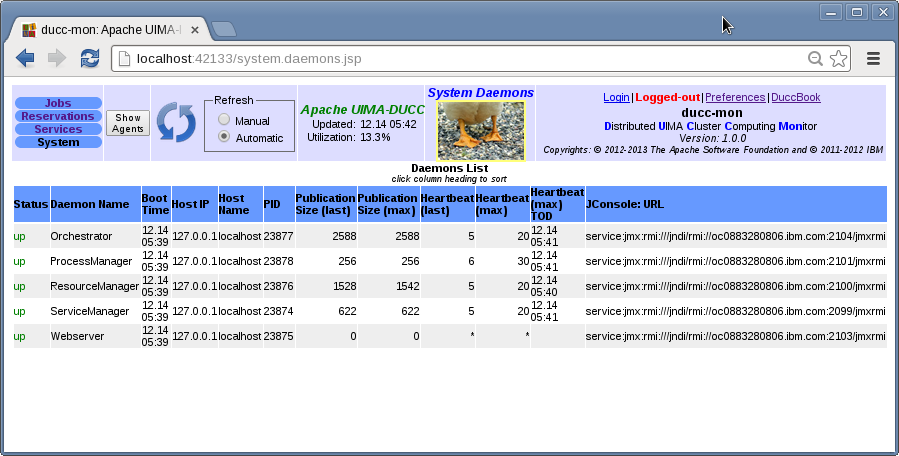
\includegraphics[width=90mm]{images/ducc-webserver/System-Daemons.png}
\caption{Sample Webserver Page}
\end{figure}

    Normally, the Web Server automatically fetches new data from {\DUCC} and updates the display.
    This is controlled by setting one of the two refresh modes:
    \begin{itemize}
      \item Manual refresh.  In this mode, the browser windows are updated only by using the
        browser's refresh button, or the {\DUCC} refresh button to the left in the header of
        each page.
      \item Automatic refresh. In this mode, the browser automatically fetches and displays
        new data.  The rate of refresh is currently fixed and cannot be configured.
    \end{itemize}
    
    There is a behavior difference between refresh and reload.
    \paragraph{Refresh}
    Refresh causes the current data on the page to be updated with the most
    current information in the Webserver's possession.  This is performed
    when the refresh button is clicked.
    \paragraph{Reload}
    Reload occurs when the enter key is pressed.  Reload causes not just the
    data to be updated but rather the entire page is replaced.
    
    Two different table styles are supported:
    \begin{itemize}
      \item Scroll, and
      \item Classic.
    \end{itemize}
    Table styles are switched using the {\em Preferences} link.

    \paragraph{Scroll Mode}  When {\em scroll table style} is the preference, a scroll bar is
    shown to the right, within the main window.  The scroll bar allows scrolling to be restricted to the data
    display, leaving column and {\DUCC} headers in place.  In this mode any column may be sorted
    simply by clicking on it.
    
    With respect to sorting, any specified sort is remembered for refresh
    but forgotten for reload.  Sorting is permitted when either manual
    or automatic refresh mode is selected.
    
    The column sort order is maintained until the page is reloaded.

	Note that not all pages have a scroll version - some only have a classic version.
	
    \paragraph{Classic Mode}  When {\em classic table style} is the preference, the
    main data may extend below the bottom of the page and it will be necessary to use the browser's scroller on the right
    to access it.  The column headers and {\DUCC} header scrolls off when doing this.  Columns
    may be sorted in this mode but it is necessary to first switch to ``Manual'' refresh mode to
    prevent browser refreshes during sorting and display of data. 
    
    With respect to sorting, any specified sort is forgotten for refresh
    and reload.  Sorting is only permitted when manual refresh mode is
    selected.
    
    The column sort order is maintained until the page is refreshed or reloaded.

\begin{figure}[ht!]
\centering
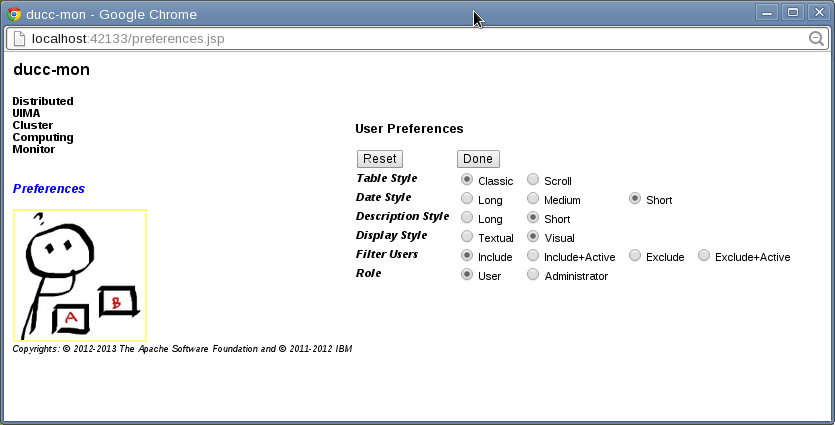
\includegraphics[width=90mm]{images/ducc-webserver/Preferences.png}
\caption{Preferences Page}
\end{figure}

% Create well-known link to this spot for HTML version
\ifpdf
\else
\HCode{<a name='DUCC_WS_COMMON'></a>}
\fi
    \section{Common Links}

        Every page contains a common header containing links and controls. The links permit navigation
        to other content at the site. The controls provide page-wise configuration of the content at
        that page.

        The following links are available on every page of the web server: 

        \begin{description}
          \item[Authentication] \hfill \\ 
            Authentication is needed in order to cancel jobs and reservations, to create a
            reservation, and to perform administration. It is not required to simply view the pages.

            \begin{itemize}
              \item Login - Authenticate and start a session with the Web Server.             
              \item Logout - Terminate the Web Server session 
            \end{itemize}

          \item[Preferences]
            The following preferences may be set:
            \begin{description}
              \item[Table Style] This selects ``scroll'' or ``classic'' display, as
                described above.
              \item[Date Style] This selects long, medium, or long formats for dates.
              \item[Description Style] This selects long or short formats for the various
                description fields.
              \item[Display Style] Choose to display text or (in some circumstances) icons.
              \item[Filter Users] This controls the ``filter'' box near the middle of
                the header on each page.  It allows various levels of inclusion and
                exclusion of active or completed work for the filtered users.
              \item[Role] This allows selection of ``User'' or ``Administrator'' roles.
                This protects registered {\DUCC} administrators from accidentally affecting
                other people's work.
            \end{description}
            
          \item[DuccBook] \hfill \\
            This is a link to the HTML version of the document you are reading.

          \item[Jobs] \hfill \\
            This navigates to the Jobs page, showing all the jobs in the system.

          \item[Reservations] \hfill \\
            This navigates to the Reservations page, showing all the reservations
            in the system and provides a button that can be used to request new reservations. 

          \item[Services] \hfill \\
            This navigates to the Services page, showing all the services in the
            system.

          \item[System] \hfill \\
            This opens a sub-menu with system-related links:
            \begin{itemize}
              \item Administration - This opens a page with administrative functions. 
              \item Broker - This shows information about the AMQ broker employed by the system. 
              \item Classes - This shows all the scheduling classes defined to the system. 
              \item Daemons - This shows the status of {\DUCC}'s management processes. 
              \item DuccBook - This manual. 
              \item Machines - This shows the status of all the {\DUCC} worker nodes. 
            \end{itemize}

            \item[Viz]
            This opens a page with a visualization of the system hosts, showing all
            scheduled work in the system.
      \end{description}              

      % Create well-known link to this spot for HTML version
      \ifpdf
      \else
      \HCode{<a name='DUCC_WS_JOBS'></a>}
      \fi
      % 
% Licensed to the Apache Software Foundation (ASF) under one
% or more contributor license agreements.  See the NOTICE file
% distributed with this work for additional information
% regarding copyright ownership.  The ASF licenses this file
% to you under the Apache License, Version 2.0 (the
% "License"); you may not use this file except in compliance
% with the License.  You may obtain a copy of the License at
% 
%   http://www.apache.org/licenses/LICENSE-2.0
% 
% Unless required by applicable law or agreed to in writing,
% software distributed under the License is distributed on an
% "AS IS" BASIS, WITHOUT WARRANTIES OR CONDITIONS OF ANY
% KIND, either express or implied.  See the License for the
% specific language governing permissions and limitations
% under the License.
% 

    \section{Jobs Page}
    \label{sec:ws.jobs-page}
        The Web Server's home page is also the Jobs page. This page has links to all the rest of the content 
        at the site and shows the status of all the jobs in the system. 
    
        The Jobs page contains the following columns: 

        \begin{description}

            \item[Id] \hfill \\
              This is the ID as assigned by {\DUCC}. This field is hyperlinked to a
              \hyperref[sec:ws-job-details]{Job Details} page for that job that shows the breakdown of
              all the processes assigned to the job and their state.
              
            \item[Start] \hfill \\
              This is the time the Job is accepted into {\DUCC}.
              
            \item[Duration] \hfill \\
              This shows two times.  In green the length of time the job has been running.  In black is
              the estimated time of completion, based on current resources and remaining work.  When
              the job completes, the time shown is the total elapsed time of the job.
                            
            \item[User] \hfill \\
              This is the userid of the job owner.
              
            \item[Class] \hfill \\
              This is the resource class the job is submitted to.
              
            \item[State] \hfill \\
              This shows the state of the job.  The normal job progression is shown below, with an
              explanation of what each state means.
              \begin{description}
                  \item[Received] - The job has been vetted, persisted, and assigned a unique ID. 
                  \item[WaitingForDriver] - The job is waiting for the Job Driver to initialize. 
                  \item[WaitingForServices] - The job is waiting for verification from the
                    Service Manager that required services are started and responding.  This may
                    cause {\DUCC} to start services if necessary.  In that even this state will
                    persist until all pre-requisite services are ready.
                  \item[WaitingForResources] - The job is waiting to be scheduled. In busy
                    systems this may require preemption of existing work.  In that case this
                    state will persist until preemption is complete.
                  \item[Initializing] - The job initializing. Usually this
                    is the UIMA-AS initialization phase.  In the default configuration, only
                    two (2) processes are allocated by the Resource Manager.  No additional
                    resources are allocated until at least one of the new processes successfully
                    completes initialization.  Once initialization is complete the Resource Manager
                    will double the number of allocated processes until the user's fair share of
                    the resources is attained.
                  \item[Running] - At least one process is now initialized and running. 
                  \item[Completing] - The last work item has completed and {\DUCC} is freeing resources.
                    If the job had many resources allocated at the time the job exited this state
                    will persist until all allocated resources are freed.
                  \item[Completed] - The job is complete. 
              \end{description}
                  
            \item[Reason or Extraordinary Status] \hfill \\

              % See this structure:
              % org.apache.uima.ducc.transport.event.common.IDuccCompletionType
              
              This field contains miscellaneous information pertaining to the job.  If the job exits
              the system for any reason, that reason is shown here.  If the job's pre-requisite
              services are unavailable (or ailing) that fact is displayed here.  If there is a
              job monitor running, that fact is shown here.  Most of the values for this field
              support ``hovers'' containing additional information about the reason.
         
              \begin{description}
                  \item[EndOfJob] - The job and completed ran with no errors. 
                  \item[Error] - All work items are processes but at least one had an error. 
                  \item[CanceledByDriver] - The Job Driver (JD) terminated the job. The reason for
                    termination is seen by hovering over the text with your mouse.
                  \item[CanceledBySystem] - The job was canceled because {\DUCC} was shutdown. 
                  \item[CanceledBySser] - The job owner or {\DUCC} administrator canceled the job. 
                  \item[Cancel Pending] - The job has been canceled and is not yet fully evicted
                    from the system.
                  \item[DriverInitializationFailure] - The Job Driver (JD) process is unable to initialize. Hover over 
                    the field with your mouse for details (if any are available), and check your JD log. 
                  \item[DriverProcessFailed] - The Job Driver (JD) process failed for some reason. Hover over the 
                    field with your mouse for details (if any), and check your JD log. 
                  \item[MonitorActive] The job has a console monitor active.  This is enabled with the
                    job's ``wait\_for\_completion'' parameter on job submission.
                  \item[ServicesUnavailable] - The job declared a dependency on one or more services, and the 
                    Service Manager (SM) cannot find or start the required service. 
                  \item[Premature] - The job was terminated for some unknown reason before all work items were 
                    processed. Check the JP logs for details. 
                  \item[ProcessInitializationFailure] - Too many processes failed during
                    initialization and the job was canceled by {\DUCC}.  Check the JP logs for the
                    reason.
                  \item[ProcessFailure] - Too many processes failed while running and {\DUCC} canceled
                    the job.  Check the JP logs for the reason.
                  \item[ResourcesUnavailable] - The Resource Manager (RM) is unable to allocate resources for 
                    the job. For non-preemptable jobs this could be because the limit on that type of allocation is 
                    reached, or all the hosts are already allocated and work cannot be preempted to make space for 
                    it. For all jobs, it could be because the job class is invalid. 
                    \item[{\em service\_name}] If there is a service name in this field it indicates the job is
                      dependent on the service but the service is not responding to the {\DUCC} Service Monitor's
                      pinger.
              \end{description}

            \item[Services] \hfill \\
              This is the number of services the job has declared dependencies on.  There is a ``hover'' that
              shows the ids of the services, if any.

            \item[Processes] \hfill \\
              This is the number of processes currently assigned to the job.

            \item[Init Fails] \hfill \\
              This is the total number of initialization failures experienced by the job. This
              field is hyperlinked to pages with log excerpts highlighting the specific failures.
              
            \item[Run Fails] \hfill \\
              This is the total number of process failures experienced by the job. This field is
              hyperlinked to pages with log excerpts highlighting the specific failures.
              
            \item[PgIn] This is the number of page-in events, over all processes, on the machines
              running the job.

            \item[Swap] This is the total swap space, over all the processes, being used by the job.

            \item[Memory] \hfill \\
              This is the declared memory size of the job
              
            \item[Total] \hfill \\
              This is the total number of work items declared by the job.
              
            \item[Done] \hfill \\
              This is the total number of work items successfully completed for the job.
              
            \item[Error] \hfill \\
              This is the total number of exceptions thrown or other errors experienced by work
              items. This field is hyperlinked to pages containing log excerpts highlighting
              the failures.
              
            \item[Dispatch] \hfill \\
              This is the total number CASs that are currently dispatched. 

              This usually represents the quantity derived from the following formula:
\begin{verbatim}              
     min( (initialized.processes * threads.per.process), (incomplete.work.items - errors) )
\end{verbatim}

              The actual number is a measured number, not a calculated number, and may differ
              slightly from the formula if the measurement is taken immediately after process
              start-up, or in the time between a work item completing and a new one being
              dispatched.
              
            \item[Retry] \hfill \\
              This is the number of CASs that were retried for any reason.  Reasons for retry
              include preemption for fair-share, work-item timeout, or error conditions.

              Note: If a work item in any process fails, the entire process is considered
              suspect, and all work-items in the process are terminated.  Work items in the
              process which did not have errors are re-dispatched (retried) to a different
              process.
              
            \item[Preempt] \hfill \\
              This is the total number of processes that have been preempted to make room for
              other work due to Fair Share.
              
            \item[Description] \hfill \\
              This is the description string from the $--$description string from submit.
            \end{description}

    \begin{figure}[ht!]
    \centering
    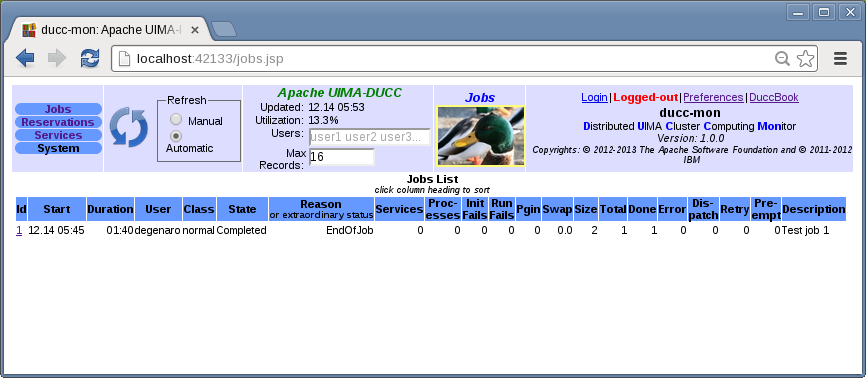
\includegraphics[width=90mm]{images/ducc-webserver/Jobs.png}
    \caption{Jobs Page}
    \end{figure}
            


      % Create well-known link to this spot for HTML version
      \ifpdf
      \else
      \HCode{<a name='DUCC_WS_JOB_DETAILS'></a>}
      \fi
      % 
% Licensed to the Apache Software Foundation (ASF) under one
% or more contributor license agreements.  See the NOTICE file
% distributed with this work for additional information
% regarding copyright ownership.  The ASF licenses this file
% to you under the Apache License, Version 2.0 (the
% "License"); you may not use this file except in compliance
% with the License.  You may obtain a copy of the License at
% 
%   http://www.apache.org/licenses/LICENSE-2.0
% 
% Unless required by applicable law or agreed to in writing,
% software distributed under the License is distributed on an
% "AS IS" BASIS, WITHOUT WARRANTIES OR CONDITIONS OF ANY
% KIND, either express or implied.  See the License for the
% specific language governing permissions and limitations
% under the License.
% 
  
    \section{Job Details Page}
    \label{sec:ws-job-details}

    This page shows details of all the processes that run in support of a job. 
    The information is divided among five tabs:
    \begin{description}
      \item[Processes] This tab contains details on all the processes for the job, both
        active, and defunct.
      \item[Work Items] This tab shows details for each individual work-item in the job.
      \item[Performance] This tab shows a performance break-down of all the UIMA analytics
        in the job.
      \item[Specification] This tab shows the job specification for the job.
      \item[Files] This tab shows the files in the log directory.
      \end{description}
      
    \subsection{Processes}
    \label{subsec:ws-processes}
    The processes page contains the following columns:
    
    \begin{description}

        \item[Id] \hfill \\
          This is the {\DUCC}-assigned numeric id of the process (not the Operating System's
          process Id). Process 0 is always the Job Driver.          

        \item[Log] \hfill \\
          This is the log name for the process. It is hyperlinked to the log itself.

        \item[Log Size] \hfill \\
          This is the size of the log in MB. If you find you have trouble viewing the log
          from the Web Server it could be because it is too big to view in the server and needs to
          be read by some other means than the Web Server.  (It is not currently paged in by 
          the Web Server, it is read in full.)

        \item[Host Name] \hfill \\
          This is the name of the host where the process ran.

        \item[PID] \hfill \\
          This is the Unix process ID (PID) of the process.

        \item[State Scheduler] \hfill \\
          % The information comes from here:
          % State Scheduler: org.apache.uima.ducc.transport.event.common.IResourceState.ResourceState

          This shows the Resource Manager state of the job. It is one of:
          \begin{description}
              \item[Allocated] - The host is currently allocated for this job by the RM.
              \item[Deallocated] - The resource manager has deallocated the shares for the job on
                this host.
          \end{description}

        \item[Reason Scheduler or extraordinary status] \hfill \\
          \phantomsection\label{itm:job-details-sched}


          % The information comes from here:
          % Reason Scheduler: org.apache.uima.ducc.transport.event.common.IResourceState.ProcessDeallocationType
          This column provides a reason for the scheduler state, when the scheduler state is other than ``Allocated''. 
          These all have ``hovers'' that provide more information
          if it is available.

            \begin{description}          
                \item[AutonomousStop] - The process terminated unexpectedly of its own accord ("crashed", or
                  simply exited.) 

                \item[Exception] - The process is terminated by the JD exception handler. 

                \item[Failed] - The process is terminated by the Agent because the JP wrapper was able to detect and 
                  communicate a fatal condition (Exception) in the pipeline.. 
                  
                \item[FailedInitialization] - The process is terminated because the UIMA initialization step failed. 
                  
                \item[Forced] - The host is preempted by RM for other work because of fair share. 
                  
                \item[JobCanceled] - The job was canceled by the user or a system administrator. 
                  
                \item[JobCompleted] - The process is canceled because of {\DUCC} restart. 
                  
                \item[JobFailure] - The job failure limit is exceeded, causing the job to be canceled by the JD.                    
                  
                \item[InitializationTimeout] - The UIMA initialization phase exceeded the configured timeout. 
                  
                \item[Killed] - The agent terminated the process for some reason. The ``Reason Agent'' field
                  should have more details in this case.
          
                \item[Stopped]	- The process was terminated by the Agent for some reason.  The hover should
                  contain more information.
                          
                \item[Voluntary] - The job is winding down, there's no more work for this host, so it stops. 
                  
                \item[Unknown] - None of the above. This is an exceptional condition, sometimes an
                  internal {\DUCC} error. Check the JP and JD logs for possible causes..
            \end{description}

          \item[State Agent] \hfill \\
          \phantomsection\label{itm:job-details-state}

          % This state comes from here:
          % State Agent: org.apache.uima.ducc.transport.event.common.IProcessState.ProcessState
            This shows the {\DUCC} Agent's view of the state of the process.
            \begin{description}
               \item[Starting] The {\DUCC} process manager as issued a request to the assigned to
                 start the process.
               \item[Initializing] The process is initializing.  Usually this means the UIMA analytic
                 pipeline (Job Process) is executing it's initialization method.
              \item[Running] The Job Process has completed the initialization phase and is ready for, 
                or actively executing work.
              \item[Stopped] The {\DUCC} Agent reports the process is stopped and (and has exited).
              \item[Failed] The {\DUCC} Agent reports the process failed with errors.  This usually
                means that UIMA-AS has detected exceptions in the pipeline and reported them
                to the Job Driver for logging.
              \item[FailedInitialization] The process died during the UIMA initialization phase.
              \item[InitializationTimeout] The process exceeded the site's limit for time spent
                in UIMA initialization.
              \item[Killed] The {\DUCC} Agent killed the process for some reason.  There are
                three reasons for this:
                \begin{enumerate}
                  \item The Job Processes failed to initialize,
                  \item The Job Process timed out during initialization,
                  \item The process Exocet's its allowed swap.
                \end{enumerate}
              \item[Abandoned] It is possible to cancel a specific process of a job.  Usually
                this is because it became ``stuck'' because of hardware failure.  It a process
                is killed in \hyperref[sec:cli.ducc-cancel]{this way}, the state is recorded as {\em Abandoned}.
            \end{description}
            
          \item[Reason Agent] \hfill \\
          \phantomsection\label{itm:job-details-agent}

          This shows extended reason information if a process exited other than having run out
          of work to do.

            \begin{description}
              \item[AgentTimedOutWatingForORState] The {\DUCC} Agent is expecting a state update
                from the {\DUCC} Orchestrator.  Timer on this wait has expired.  This usually 
                indicates an infrastructure or communication problem.
              \item[Croaked] The process exited for no good or clear reason, it simply vanished.
              \item[Deallocated] WHAT IS THIS?
              \item[ExceededShareSize] The process exceeded it's declared memory size.
              \item[ExceededSwapThreshold] The process exceeded the configured swap threshold.
              \item[FailedInitialization] The process was terminated because the UIMA 
                initialization step failed.
              \item[InitializationTimeout] The process was terminated because the UIMA initialization
                step took too long.
              \item[JPHasNoActiveJob] This is set when an agent looses connectivity while its
                JPs are running. The job finishes (stopped or killed). The agent regains
                connectivity. The OR publish no longer includes the job but the agent still has
                processes running for that job. The agent kills ghost processes with the reason:
                JPHasNoActiveJob.
              \item[LowSwapSpace] The process was terminated because the system is about to run
                out of swap space.  This is a preemptive measure taken by {\DUCC} to avoid exhaustion
                of swap, to effect orderly eviction of the job before the operating system starts
                its own reaping procedures.
              \item[AdministratorInitiated] The process was canceled by an administrator.
              \item[UserInitated] The process was canceled by the owning user.
            \end{description}
                    
          \item[Exit] \hfill \\
            The process exit code or signal.
            
          \item[Time Init] \hfill \\
            This is the clock time this process spent in initialization.
            
          \item[Time Run] \hfill \\
            This is the clock time this process spent in executing, not including
            initialization.
            
          \item[Time GC] \hfill \\
            This is amount of time spent in Java Garbage Collection for the process.
            
          \item[PgIn] \hfill \\
            This is the number of page-in events on behalf of the process.

          \item[Swap] \hfill \\
            This is the amount of swap space on the machine being consumed by the process.

          \item[\%CPU] \hfill \\
            Current CPU percent consumed by the process.  This will be $>$ 100\% on 
            multi-core systems if more than one core is being used.  Each core contributes
            up to 100\% CPU, so, for example, on a 16-core machine, this can be as high
            as 1600\%.
            
          \item[RSS] \hfill \\
            The amount of real memory being consumed by the process (Resident Storage Size)
            
          \item[Time Avg] \hfill \\
            This is the average time in seconds spent per work item in the process.
            
          \item[Time Max] \hfill \\
            This is the minimum time in seconds spent per work item in the process.
            
          \item[Time Min] \hfill \\
            This is the minimum time in seconds spent per work item in the process.
            
          \item[Done] \hfill \\
            This is the number of work items processed in this process.
            
          \item[Error] \hfill \\
            This is the number of exceptions processing work items in this process.
                      
          \item[Dispatch] \hfill \\
            The number of work items currently dispatched.
              
          \item[Retry] \hfill \\
            This is the number of work items that were retried in this process for any reason, excluding
            preemption.
            
          \item[Preempt] \hfill \\
            This is the number of work items that were preempted from this process, if
            fair-share caused preemption.
            
          \item[JConsole URL] \hfill \\
            This is a URL that can be used to connect via JMX to the processes, e.g. via
            jconsole.

      \end{description}
      
    \begin{figure}[ht!]
    \centering
    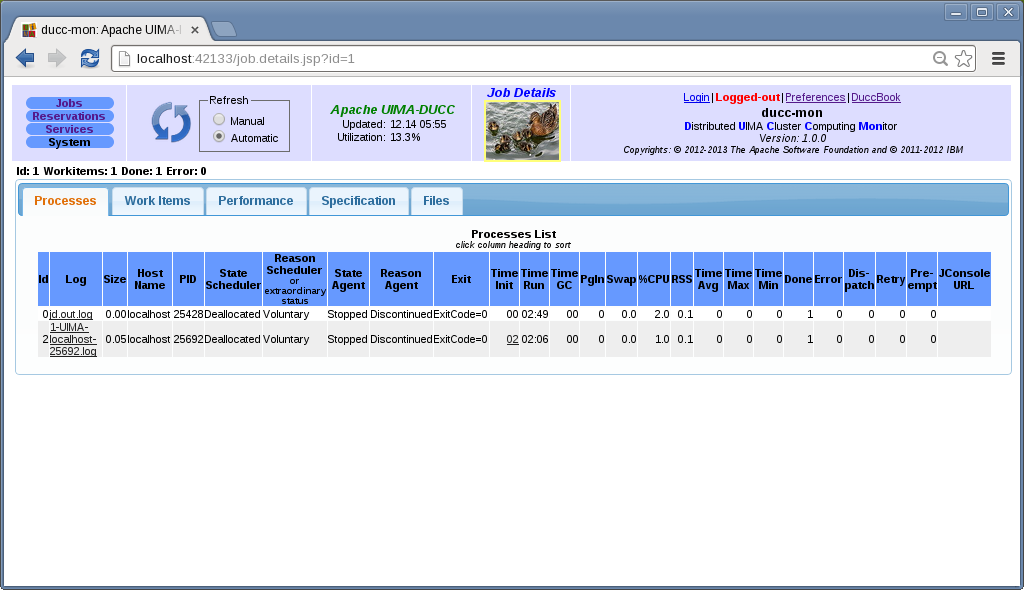
\includegraphics[width=90mm]{images/ducc-webserver/Job-Details-Processes.png}
    \caption{Processes Tab}
    \end{figure}
    
   \subsection{Work Items}
   \label{subsec:ws-work-items}
   This tab provides details for each individual work item.  Columns include:

   % The data comes from here: org.apache.uima.ducc.common.jd.files.IWorkItemState.State    
   \begin{description}
     \item[SeqNo]  \hfill \\
       This is the sequence work items are fetched from the Collection Reader's
       getNext() method by the {\DUCC} Job Driver.
     \item[Id]  \hfill \\
       This is the name of the work item.
     \item[Status]  \hfill \\
       The is the current state of the work item.  
       States include:
       \begin{description}
         \item[ended] The work item is complete.
         \item[error] The work item ended with errors.
         \item[lost] The work item was queued to ActiveMQ but never dequeued by
         any Job Process.
         \item[operating] The work item is current being executed.
         \item[retry] The work item is being retried.
         \item[start] The work item has been picked up for execution and {\DUCC} is waiting
           for confirmation that it is running.
         \item[queued] The work item has been queued to ActiveMQ but not picked up by any
           Job Process yet.
       \end{description}
       If a work item has not yet been retrieved from the Collect Reader it does not show
       on this page.
     \item[Delivery Time (sec)]  \hfill \\
       The time spent in getting a work item from the Job Driver to a Job Process.
     \item[Processing Time (sec)]  \hfill \\
       The time spent processing the work item.
     \item[Investment Time (sec)]  \hfill \\
       The time spent processing the work item during the current epoch.
     \item[Host (IP)]  \hfill \\
       The host IP where the work item was processed.
     \item[Host (Name)]  \hfill \\
       The host name where the work item was processed.
     \item[PID]  \hfill \\
       The Unix Process Id that the work item was processed in.
   \end{description}
    
    \begin{figure}[ht!]
    \centering
    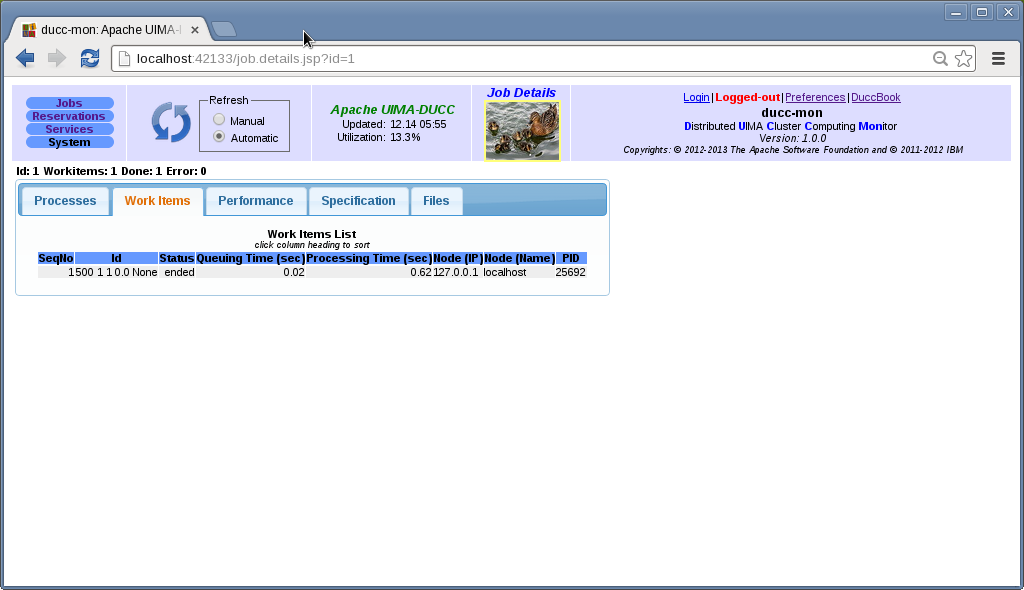
\includegraphics[width=90mm]{images/ducc-webserver/Job-Details-WorkItems.png}
    \caption{Work Items Tab}
    \end{figure}  

   \subsection{Performance}
   \label{subsec:performance}
   This tab shows performance summaries of all the pipeline components.  The statistics
   are aggregated over all instances of each component in each process of the job.
   
   \begin{description}
     \item[Name]  \hfill \\
       The short name of the analytic.  The full name is shown in the command-line
       tool \hyperref[sec:cli.ducc-perf-stats]{ducc\_perf\_stats}
     \item[Total]  \hfill \\
       This is the total time in days, hours, minutes, and seconds taken by each
       component of the pipeline.
     \item[\% of Total]  \hfill \\
       This is the percent of the total usage consumed by this analytic.
     \item[Avg]  \hfill \\
       This is the average time spent by all the instances of the analytic.
     \item[Min]  \hfill \\
       This is the minimum time spent by any instance of the analytic.
     \item[Max]  \hfill \\
       This is the maximum time spent by any instance of the analytic.
   \end{description}
    
    \begin{figure}[ht!]
    \centering
    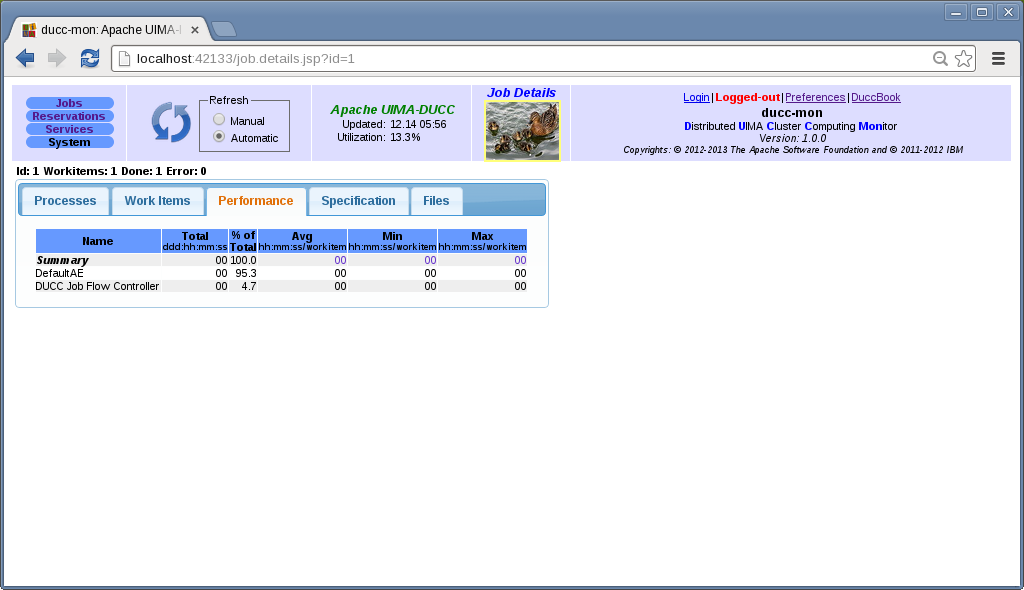
\includegraphics[width=90mm]{images/ducc-webserver/Job-Details-Performance.png}
    \caption{Performance Tab}
    \end{figure}  
       
   \subsection{Specification}
   This tab shows the full job specification in the form of a Java Properties
   file.  This will include all the parameters specified by the user, plus those
   filled in by {\DUCC}.
    
    \begin{figure}[ht!]
    \centering
    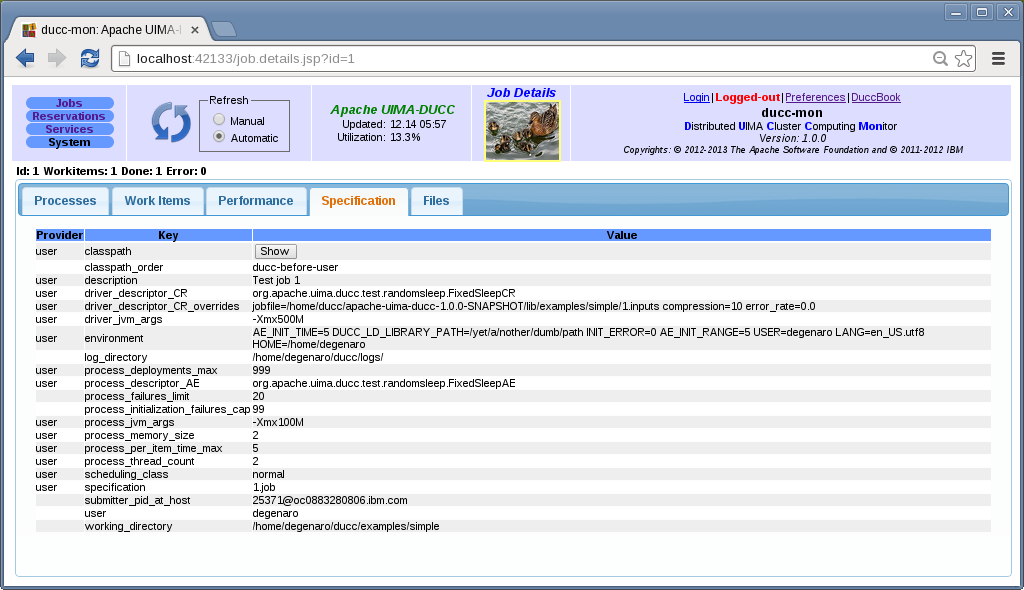
\includegraphics[width=90mm]{images/ducc-webserver/Job-Details-Specification.png}
    \caption{Specification Tab}
    \end{figure}  
    
   \subsection{Files}
   This tab shows the files in the log directory.


      % Create well-known link to this spot for HTML version
      \ifpdf
      \else
      \HCode{<a name='DUCC_WS_RESERVATIONS'></a>}
      \fi
      % 
% Licensed to the Apache Software Foundation (ASF) under one
% or more contributor license agreements.  See the NOTICE file
% distributed with this work for additional information
% regarding copyright ownership.  The ASF licenses this file
% to you under the Apache License, Version 2.0 (the
% "License"); you may not use this file except in compliance
% with the License.  You may obtain a copy of the License at
% 
%   http://www.apache.org/licenses/LICENSE-2.0
% 
% Unless required by applicable law or agreed to in writing,
% software distributed under the License is distributed on an
% "AS IS" BASIS, WITHOUT WARRANTIES OR CONDITIONS OF ANY
% KIND, either express or implied.  See the License for the
% specific language governing permissions and limitations
% under the License.
% 

\section{Reservation Page}
\label{sec:ws-reservations}

This page shows details of all reservations.  There are two types of reservations: {\em managed}
and {\em unmanaged}.

A {\em managed reservation} is a reservation whose process is fully managed by {\DUCC}.  This process
is any arbitrary process and is submitted with the
\hyperref[sec:cli.ducc-process-submit]{ducc\_process\_submit} CLI.  The lifetime of the reservation
starts at the time {\DUCC} assigns a unique ID, and ends when the process terminates for any reason.

An {\em unmanaged reservation} is essentially a sandbox for the user.  {\DUCC} starts no processes
in the reservation and manages none of the processes which run on that host.  The lifetime of the
reservation starts at the time {\DUCC} assigns a unique ID, and ends when the submitter or system
administrator cancels it.  {\em Managed reservations} can potentially last an indefinite
period of time.

The Reservations page contains the following columns: 
\begin{description}

\item[Id] \hfill \\
  This is the unique {\DUCC} numeric id of the reservation as assigned when the reservation is made.
  If this is a {\em managed} reservation, the ID is hyperlinked to a
  \hyperref[sec:ws-managed-reservation-details]{Managed Reservation Details} page with extended
  details on the process running in the reservation.

\item[Start] \hfill \\
  This is the time the reservation was mode.
  
\item[Duration] \hfill \\
  A time in green is the length of time the active reservation has been assigned.  
  A time in black is the length of time the completed reservation was assigned. 
  
\item[User] \hfill \\
  This is the userid if the person who made the reservation.
  
\item[Class] \hfill \\
  This is the scheduling class used to schedule the reservation.
  
\item[Type] \hfill \\
  This is the reservation type, {\em managed} or {\em unmanaged}, as described 
  \hyperref[sec:ws-reservations]{above}.

\item[State] \hfill \\
  % 1. org.apache.uima.ducc.transport.event.common.IDuccState
  This is the status of the reservation. Values include: Received - Reservation
  has been vetted, persisted, and assigned unique Id.
  \begin{description}
  \item[Assigned] - The reservation is active. 
  \item[Completed] - The reservation has been terminated.
  \item[Received] - The Reservation has been vetted, persisted, and assigned a unique ID.
  \item[WaitingForResources] - The reservation is waiting for the Resource Manager to find and 
    schedule resources. 
  \end{description}

\item[Reason] \hfill \\

  % 2. org.apache.uima.ducc.transport.event.common.IDuccCompletionType

  If a reservation is not active, this shows the reason.  Note that for
  {\em unmanaged reservations}, even if the user has processes running in the
  reservation, {\DUCC} does NOT attempt to terminate those processes (hence, ``unmanaged''.)

  For {\em managed reservations}, {\DUCC} does terminate the associated process.

  \begin{description}
  \item[CanceledBySystem] - In the case of the special JobDriver reservation, this is
    canceled by {\DUCC} and reestablished on reboot; hence the state is a result of {\DUCC}
    having been restarted.

    In all other cases, it is a result of {\DUCC} being restarted {\em COLD}.  When
    {\DUCC} is started {\em COLD}, all previous reservations are canceled.  (When {\DUCC}
    is started {\em WARM}, the default, previous reservations are preserved.)
  \item[CanceledByAdmin] - The {\DUCC} administrator released the reservation. 
  \item[CanceledByUser] - The reservation owner released the reservation. 
  \item[ResourcesUnavailable] - The Resource Manager was unable to find free or freeable resources 
    match the resource request. 
  \item[ProgramExit] - The reservation is a {\em managed} reservation and the associated
    process has exited.
  \end{description}

\item[User Processes] This is the number of processes owned by the user running in all
  shares of the reservation.  
  
  Note that even for {\em unmanaged} reservations, the {\DUCC} agent tracks processes owned
  by the user and reports on them.  This allows better identification and management of
  abandoned reservations.
          
\item[PgIn] This is the number of page-in events for the managed reservation.

\item[Swap] This is the total swap space for the managed reservation.

\item[Memory] \hfill \\
  The memory size in GB of the each allocated unit.  This is the amount of memory that
  was {\em requested}.  In the case of RESERVE policy reservations, that actual memory
  of the reserved machine may be greater.
  
\item[Host Names] \hfill \\
  The host names of the machines where the resources are allocated.
  
\item[Description] \hfill \\
  This is the description string from the --description string from submit.
\end{description}

    \begin{figure}[ht!]
    \centering
    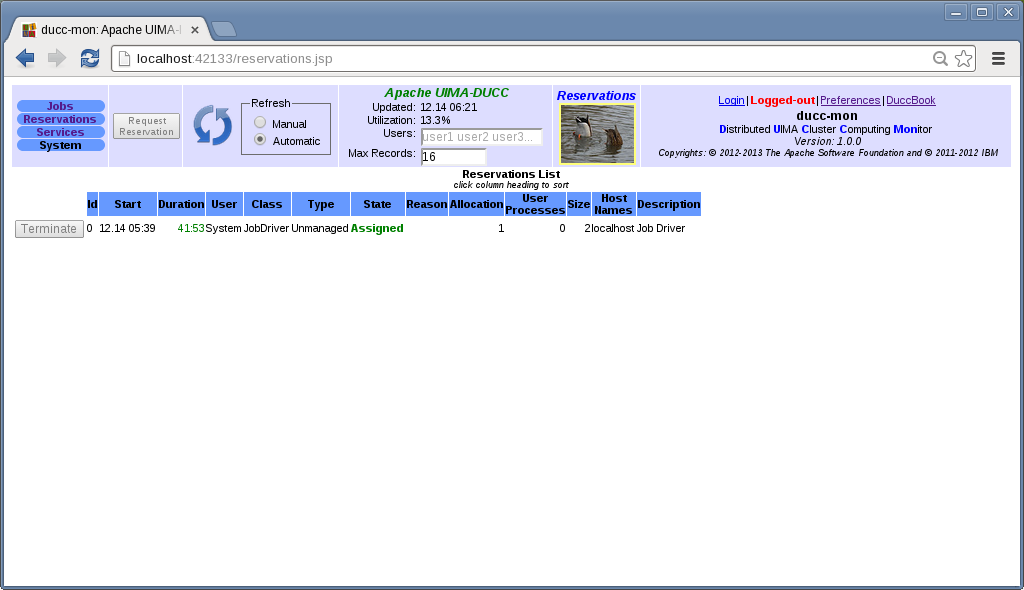
\includegraphics[width=90mm]{images/ducc-webserver/Reservations.png}
    \caption{Reservations Page}
    \end{figure}


      % Create well-known link to this spot for HTML version
      \ifpdf
      \else
      \HCode{<a name='DUCC_WS_RESERVATIONS_DETAILS'></a>}
      \fi
      % 
% Licensed to the Apache Software Foundation (ASF) under one
% or more contributor license agreements.  See the NOTICE file
% distributed with this work for additional information
% regarding copyright ownership.  The ASF licenses this file
% to you under the Apache License, Version 2.0 (the
% "License"); you may not use this file except in compliance
% with the License.  You may obtain a copy of the License at
% 
%   http://www.apache.org/licenses/LICENSE-2.0
% 
% Unless required by applicable law or agreed to in writing,
% software distributed under the License is distributed on an
% "AS IS" BASIS, WITHOUT WARRANTIES OR CONDITIONS OF ANY
% KIND, either express or implied.  See the License for the
% specific language governing permissions and limitations
% under the License.
% 
\section{Managed Reservation Details Page}
\label{sec:ws-managed-reservation-details}

This page shows details of the processes which run in a managed reservation.  The
information is divided between three tabs:

   \begin{description}
       \item[Processes] This tab contains details on all the processes contained in the
         reserved space.
       \item[Specification] This tab shows the specification for the process.
       \item[Files] This tab shows the files in the log directory.
   \end{description}  

   \subsection{Processes}
   \label{sec:ws-manres-processes}

   The processes page contains the following columns:
   \begin{description}
      \item[Id] \hfill \\
        This is the {\DUCC}-assigned numeric id of the process.  This format of this
        id is two numbers:
\begin{verbatim}
    RESID.SHAREID
\end{verbatim}
        Here, the {\em RESID} is the reservation ID.  The {\em SHAREID} is the 
        share ID assigned by the Resource Manager.  Together these form a unique
        ID for each process that runs in the reservation.
        
        Note: The current version of {\DUCC} supports only one process per managed
        reservation.  Future versions are expected to support multiple processes
        within a single managed reservation.
        
      \item[Log] \hfill \\
        This is the log name for the process. It is hyperlinked to the log itself.
        
      \item[Log Size] \hfill \\
        This is the size of the log in MB. If you find you have trouble viewing the log
        from the web server it could be because it is too big to view in the browser.
        
      \item[Host Name] \hfill \\
        This is the name of the host where the process is running (or ran).
        
      \item[PID] \hfill \\
        This is the Unix process ID (PID) of the process.
        
      \item[State Scheduler] \hfill \\
        This shows the Resource Manager state of the job. It is one of:
        
        \begin{description}
            \item[Allocated] - The host is still allocated for this job by the RM.
            \item[Deallocated] - The resource manager has deallocated the shares for the job on
              this host.
        \end{description}
        
      \item[Reason Scheduler or Extraordinary Status] \hfill \\
        These are the same as for the \hyperref[itm:job-details-sched]{job details.}

      \item[State Agent] \hfill \\
        These are the same as for the \hyperref[itm:job-details-state]{job details.}

      \item[Reason Agent] \hfill \\
        These are the same as for the \hyperref[itm:job-details-agent]{job details.}

      \item[Exit] \hfill \\
        The process exit code or signal.

      \item[Time Run] \hfill \\
        The current duration of the reservation, or total duration if it has 
        terminated.
      
      \item[PgIn] \hfill \\
        This is the number of page-in events on behalf of the process.

      \item[Swap] \hfill \\
        This is the amount of swap space on the machine being consumed by the process.
      
      \item[\%CPU] \hfill \\
        Current CPU percent consumed by the process.  This will be $>$ 100\% on 
        multi-core systems if more than one core is being used.  Each core contributes
        up to 100\% CPU, so, for example, on a 16-core machine, this can be as high
        as 1600\%.
      
      \item[RSS] \hfill \\
        The amount of real memory being consumed by the process (Resident Storage Size)

   \end{description}

   \subsection{Specification}
   \label{sec:ws-service-specification}
   This tab shows the full managed reservation specification in the form of a Java Properties
   file.  This will include all the parameters specified by the user, plus those
   filled in by {\DUCC}.
        
   \subsection{Files}
   This tab shows the files in the log directory.
        

      % Create well-known link to this spot for HTML version
      \ifpdf
      \else
      \HCode{<a name='DUCC_WS_SERVICES'></a>}
      \fi
      % 
% Licensed to the Apache Software Foundation (ASF) under one
% or more contributor license agreements.  See the NOTICE file
% distributed with this work for additional information
% regarding copyright ownership.  The ASF licenses this file
% to you under the Apache License, Version 2.0 (the
% "License"); you may not use this file except in compliance
% with the License.  You may obtain a copy of the License at
% 
%   http://www.apache.org/licenses/LICENSE-2.0
% 
% Unless required by applicable law or agreed to in writing,
% software distributed under the License is distributed on an
% "AS IS" BASIS, WITHOUT WARRANTIES OR CONDITIONS OF ANY
% KIND, either express or implied.  See the License for the
% specific language governing permissions and limitations
% under the License.
% 

      \section{Overview.} 
      A DUCC service is defined by the following two criteria:
      \begin{itemize}
          \item A service is one or more long-running processes that await requests
            and return something in response. 
          \item A service that is managed by DUCC is accompanied by a small program called a
            ``pinger'' that the DUCC Service Manager uses to gauge the availability and health of
            the service.  This pinger must always be be present. DUCC will supply a default
            pinger for UIMA-AS services if none is specified.
            
            Users may supply their own ``pingers'' by supplying a Java class that implements
            the pinger API.  This is referred to as a ``custom'' pinger in this document. 
            There are a number of service registration options which  allow
            specification and parametrization of custom pingers.

          \end{itemize}
      The pinger API enables the following functions for custom pingers:
      \begin{itemize}
      \item increase and decrease the number of service instances, 
      \item manage failure restart policies, 
      \item enable and disable service autostart, 
      \item notify the Service Manager of the date of last use of a service, 
      \item notify the Service Manager of the health and availability of a service, 
      \item returns a string for display in the DUCC Web server to show relevant service information
      \end{itemize}
      

      A service is usually a UIMA-AS service, but DUCC supports any arbitrary process as a service.

      The DUCC Service Manager implements several high-level functions:
      
      \begin{itemize}
          \item Ensure services are available for jobs before allowing the jobs to start.
          \item Enable fast-fail for jobs which reference services which are unavailable.
          \item Start a service when it is referenced by a job, and stop it when no longer needed.
          \item Optionally start a service when DUCC is booted.
          \item Insure services remain operational across failures.
          \item Report service failures.
          \item Run service pingers and respond to the pinger API as needed.
       \end{itemize}

       When work enters the system with a declared dependency on a service, one of the following
       actions is taken:
       \begin{itemize}
          \item If the service is not registered, the work request is automatically canceled (to avoid
            wasting resources on a job that is known cannot succeed.)
          \item If the service registered but not running, the Service Manager attempts to start it; the job
           remains queued until the service is started and its pinger reports good health.
         \item If the service exists but cannot be started, the remains queued and error
             status is shown in the web server.  Once the service is working again the
             work is allowed to proceed.  (Jobs already running are not directly affected, unless they
             also cannot access the service.)
           \item If the service processes are running but the pinger reports failure contacting the service,
               the work remains queued with error status shown in the webserver.  Once the service
               pinger indicates the service is functional again the work is allowed to proceed.
       \end{itemize}
                
    \section{Service Types.}
    \label{sec:services.types}
      DUCC supports two types of services: UIMA-AS and CUSTOM:
      
      \begin{description}
          \item[UIMA-AS] This is a normal UIMA-AS service. DUCC fully supports all aspects of UIMA-AS
            services with minimal effort from developers.  A default pinger is supplied by DUCC
            for UIMA-AS services.  It is legal to define a custom pinger for a UIMA-AS service.
            
          \item[CUSTOM] This is any arbitrary service.  Developers must provide a custom pinger
            and declare the pinger in the service registration.            
      \end{description}

      DUCC also supports services that are not managed by DUCC.  These are known as {\em ping-only}
      services.  The registration for a ping-only service contains only keywords needed to support a
      pinger, which communicates with the non-DUCC service.  Ping-only services must
      be defined as custom services; there is no default pinger provided for ping-only services.

      \section{Service Instance IDs}
      \label{sec:service.service.ids}
      DUCC 2.0.0 introduces support for constant service instance IDs.  As a service is being
      started, the SM assigns monotonically increasing IDs to each service instance, starting
      with ID 0, up the the maximum number of instances started.

      If an instance exits unexpectedly, the SM re-spawns it (unless a failure threshold has been
      exceeded).  The new instance is assigned the same instance ID as the instance it replaces.
      This insures that, for example, instance ``three'' is always started as instance ``three'',
      maintained constant over failures and SM restarts.

      The instance ID is communicated to the process through the environment with the key
      {\tt DUCC\_SERVICE\_INSTANCE}.  This key may also be used in service registrations if it
      is desired to pass the instance ID via parameters of some sort.  For example:
\begin{verbatim}
        service_jvm_args   -DSERVICE_ID=${DUCC_SERVICE_INSTANCE}
        process_executable_args -i ${DUCC_SERVICE_INSTANCE}
\end{verbatim}

      \section{Service References and Endpoints} 
      \label{sec:service.endpoints}
      Services are identified by an entity called a {\em service endpoint}.  Jobs and other
      services use the registered service endpoint to indicate dependencies on specific
      services.

      A service endpoint is of the form 
\begin{verbatim}
      <service-type>:<unique id>
\end{verbatim}
      
      The {\em service-type} must be either UIMA-AS or CUSTOM.
      
      The {\em unique id} is any string needed to ensure the service is
      uniquely named.  For UIMA-AS services, the unique ID must be the same as the
      service endpoint specified in service's DD XML descriptor.  The UIMA-AS
      service endpoint is always of the form:
\begin{verbatim}
      queue-name:broker-url
\end{verbatim}
      where {\em queue-name} is the name of the ActiveMQ queue used by the service, and {\em broker-url}
      is the ActiveMQ broker URL.  Sample DUCC Service endpoints: 
\begin{verbatim}
      UIMA-AS:WikipediaSearchServices:tcp://broker1:61616
      UIMA-AS:GoogleSearchServices:http://broker2:61618
\end{verbatim}

      Jobs or other services may register dependencies on specific services by listing one or more
      service endpoints int their specifications. See the 
      \hyperref[sec:cli.ducc-submit]{\em job } and 
      \hyperref[sec:cli.ducc-services]{\em services } CLI descriptions for details.
                       
      A service is registered with DUCC using the \hyperref[sec:cli.ducc-services]{ducc\_services}
      API/CLI. Service registrations are persisted by DUCC and last over DUCC and cluster restarts.

      \section{Service Management Policies}
      \label{sec:service.management-policy}

      The Service Manager implements these policies for managing services:
      \begin{description}

         \item[Autostarted Services] An autostarted service is automatically started when the DUCC
           system is first booted.  If an instance should die, DUCC automatically restarts the
           instance and continually maintains the registered number of service instances.

           By default, to handle fatal errors in {\em autostarted} services, The Service Manager maintains a time
           window in which only a specific number of instance failures may occur.  If the number of
           failures within that window of time is excessive DUCC will set a {\em disabled} flag and
           no longer restart instances.  Instance which do not fail are left running.  The {\em
             disabled} flag must be manually reset once the problem is resolved before new instances
           can be started.

           The default failure policy is implemented in the service pinger.. Service
           owners may redefine the default policy by supplying their own pingers for a service.
          
         \item[Reference-started Services] A reference-started service is a registered service that
           is started only when referenced by another job or service. If the service is already
           started, the dependent job/service is marked ``Services Available'' and can be scheduled.. If
           not, the service registry is checked and if a matching enabled service is found, it is 
           started by DUCC.  While the service is being started, jobs are held ``Waiting For Services''
           to ensure the service is viable. Once the service has completed initialization and the pinger 
           indicates it is viable, all work waiting on it is then marked ``Services Available'' and
           started.  
          
           To handle fatal errors in {\em reference-started} services, The Service Manager maintains
           a time window in which only a specific number of instance failures may occur.  If the
           number of failures within that window of time is excessive DUCC will set a {\em disabled}
           flag and no longer restart instances.  Instance which do not fail are left running. The
           {\em disabled} flag must be manually reset once the problem is resolved before new
           instances can be started.  This default policy may be overridden by custom pingers.
           
           When the last job or service that references the on-demand service exits, a timer is
           established to keep the service alive for a while, in anticipation that it will be needed
           again soon.  When the keep-alive timer expires, and there are no more dependent jobs or
           services, the reference-started service is automatically stopped to free up its resources
           for other work.  The time the service is allowed to remain alive is known as its
           {\em linger} time and can be controlled with the {\em service\_linger} keyword in the
           service registration.

        \item[Manually started services] A service may be started via the CLI if it is not
          already running and in the absence of references by other work.  A service which is
          manually stared by the CLI can only be stopped manually by the CLI.

          As is the case for {\em autostarted} and {\em reference-started} services, failed 
          instances will be restarted unless the number of failures within the failure window
          is exceeded and the {\em disable} flag is set.  

        \item[Ping-Only Services] 
          \phantomsection\label{subsub:services.ping-only}
          Ping-only services consist of only
          a ping thread.  The service itself is not managed in any way by DUCC.  This is useful for
          managing dependencies on services that are not under DUCC control: the pinger is used
          to assess the viability of the external service and prevent dependent jobs from
          continuing if the service is unavailable.

          Only CUSTOM services may be defined as ping-only services in this version of DUCC.

      \end{description}

      \paragraph{Dynamically Changing Service Policies}
      A service may be {\em stopped}; that is, no instances are running.  This state can occur
      if the service has experienced too many errors within its failure window, in which case
      the service is {\em disabled}, or because the service is not {\em autostarted} or {\em referenced} by
      other work. 

      If a manual {\em stop} is issued the service will be automatically {\em disabled} to insure it
      cannot be restarted (by {\em reference} or at boot with {\em autostart}) without manual
      intervention.

      In all cases, if a service is {\em disabled}, it must be manually {\em enabled} using the CLI.

      It is possible, via the CLI, to dynamically switch any service from any management policy
      to any other policy, as shown in the following table.

      See the \hyperref[sec:cli.ducc-services]{\em Service CLI } reference for details on the various 
      commands described in this section.

      \begin{tabular}{| l | l | p{6cm} | p{6cm} |}
        \hline
        Current Mode & Desired Mode & Action & Notes \\
        \hline
        \hline
        Autostart    & Manual       & Use CLI to modify registration to {\em autstart false}. & Service does not stop until requested by CLI. Service will not start at DUCC boot.\\
        \hline
        Autostart    & Reference    & Use CLI to modify registration to {\em autostart false} and {\em observe references}. & Service stops  after last reference exits, plus {\em linger} time.\\
        \hline
        Autostart    & {\em Stopped} & Use CLI to stop the service. & The CLI stop will by necessity {\em disable} the service to insure it remains stopped. \\
        \hline
        Reference    & Autostart    & Use CLI to modify registration to {\em autostart true}. & Service continues to run after last reference exits.  Service always started at DUCC boot. \\
        \hline
        Reference    & Manual       & Use CLI to {\em ignore references}. & Service continues to run after last reference exits. \\
        \hline
        Reference    & {\em Stopped} & Use CLI to stop the service. & The CLI stop will by necessity {\em disable} the service to insure it remains stopped. \\
        \hline
        Manual       & Autostart    & Use CLI to modify registraiton to {\em autostart true}. & Service will be started on DUCC boots. \\
        \hline
        Manual       & Reference    & Use CLI to {\em observe references}. & Service will stop after last referencing job exits, plus {\em linger} time.. \\
        \hline
        Manual      & {\em Stopped} & Use CLI to stop the service. & The CLI stop will by necessity {\em disable} the service to insure it remains stopped. \\
        \hline
        {\em Stopped} & Autostart    & Use CLI to modify registration to {\em autostart true}. & Service will start immediately. It may be necessary to {\em enable} the service as well.\\
        \hline
        {\em Stopped} & Reference    & Submit a job or service that references the service. & It may be necessary to {\em enable} the service as well. 
                                       The service will stop after the last referencing work exits, plus {\em linger}.  \\
        \hline
        {\em Stopped} & Manual       & Use CLI to start the service. &  The CLI start will also {\em enable} the service if necessary. \\
        \hline
      \end{tabular}
      
      \section{Service Pingers}
      \label{sec:service.pingers}
      A service pinger is a small program that queries a service on behalf of the DUCC Service
      Manager.  A default pinger is provided for UIMA-AS services and provides the following
      functions:
      \begin{itemize}
        \item Determine if the service is responsive by issuing a UIMA-AS ``get-meta'' call 
          to the service.
        \item Determine the health of the service by issuing a JMX call to the UIMA-AS broker
          to collect queueing statistics.
        \item Manage the failure window of the service.
        \item Returns a string with basic ActiveMQ statistics about the service, or
          error information if the service is deemed unusable.
        \item Returns date of last use of the service (as determined by presence or
          absence of service producers attached to the service queue).
      \end{itemize}

      Users may supply their own pingers.  The following additional functions are available for
      pingers.  Note that a {\em custom} pinger MAY be supplied for UIMA-AS services, and
      MUST be supplied for CUSTOM services.  Custom pingers use the Service Manager's
      ``pinger'' API to perform the following tasks:
      \begin{itemize}
        \item Inform the Service Manager if the service is viable.
        \item Inform the Service Manager if the service is ``healthy''.  Service ``health''
          is a heuristic used in the DUCC Web server as an alert that a service 
          is responding but may
          not be performing well.
        \item Manage service failure policies. Default failure-window policy is
          provided to all pingers by the DUCC API handler (optional).
        \item Return a string describing current service status, for use by the
          web server.
        \item Instruct the service manager to increase the number of instances (optional).
        \item Instruct the service manager to decrease the number of instances (optional).
        \item Enable and disable the services autostart flag (optional).
        \item Enable logging of a service's health and state (optional).
        \item Return date of last-use to the Service Manager for display in the
          webserver (optional).
      \end{itemize}

      \subsection{The Pinger API}

      Pingers are passed static information about the service at pinger-initialization
      time, and subsequently, current state of the service is provided on each call (ping).

      Information provided at initialization follows.  Most of this is
      provided in fields in the {\em AServicePing} base class.  See the Javadoc for 
      specific field names and types.

      \subsubsection{Pinger Initialization Data}
      Data provided once, during pinger initialization, includes:
      \begin{description}
        \item[Arguments] This is the {\em service\_ping\_arguments} string from the
          service registration.
        \item[Endpoint] This is the CUSTOM:string or UIMA-AS:string endpoint provided
          in the service registration.
        \item[Monitor Rate] This is the rate at which the pinger will be called by
          the SM, as provided in DUCC's configuration.
        \item[Service ID] This is the \hyperref[sec:service.service.ids]{unique numeric service ID} assigned to the service
          by DUCC.
        \item[Log Enabled] Whether the service log is enabled, as specified by the
          {\em service\_ping\_dolog} registration parameter.
        \item[Maximum Allowed Failures] This is the value of the {\em instance\_failures\_limit}
          parameter, provided by DUCC configuration and optionally overridden by the
          service registration.
        \item[Instance Failure Window] This is the value of the {\em instance\_failures\_window}
          parameter, provided by DUCC configuration and optionally overridden by the
          service registration.
        \item[Autostart Enabled] This indicates whether the service registration currently
          has the {\em autostart} flag enabled.
        \item[Last Use] This is the time of last known use of the service, persisted and
          maintained over SM restarts.  It is 0 if unknown or the service has never been
              used.
      \end{description}
        
      \subsubsection{Pinger Dynamic Data}

      Dynamic information provided to the pinger in each call (ping) consists of:
      \begin{description}
        \item[All Instance Information] This is an array consisting of the unique integer
          IDS of all running processes implementing the service.  This includes instances
          which may not be currently viable for some reason (still initializing, for example).

        \item[Active Instance Information] This is an array consisting of the unique integer
          IDS of all running processes implementing the service.  This is a subset of 
          ``All Instance Information'' and includes only the service instances that are advanced
          to Running state.

        \item[Reference Information] This is an array consisting of the unique integer
          IDS of all DUCC work (Jobs, other Services, etc) currently referencing the
          service.  
          
        \item[Autostart Enabled] The current state of the service's autostart flag.
          
        \item[Run Failures] This is the total number of instance failures for the 
          service since the last start of the SM.
      \end{description}

      Only a Java API is supported.

      \subsection{Declaring a Pinger in A Service}

      The following registration options are used for declaring and configuring pingers.  Any of these
      may be dynamically modified with the service CLI's {\em$--$modify} option.  Dynamically changing
      these causes the current pinger to be terminated and restarted with the new configuration.  See
      \hyperref[sec:cli.ducc-services]{ducc\_services} for details of the options:
      \begin{itemize}
        \item service\_ping\_arguments
        \item service\_ping\_class
        \item service\_ping\_classpath
        \item service\_ping\_jvmargs
        \item service\_ping\_timeout
        \item service\_ping\_dolog
        \item instance\_failures\_window
        \item instance\_failures\_limit
      \end{itemize}

      
      \subsection{Implementing a Pinger}
      Pingers must implement the class {\tt org.apache.uima.ducc.cli.AServicePing}.  See the
      Javadoc for the details of this class.

      Below is a sample CUSTOM pinger for a hypothetical service that returns four integers in
      response to a ping.  It illustrates simple use of the three required methods, {\em init()},
      {\em stop()}, and {\em getStatistics()}.

      \begin{figure}[H]
\begin{verbatim}
import java.io.DataInputStream;
import java.io.InputStream;
import java.net.Socket;
import org.apache.uima.ducc.cli.AServicePing;
import org.apache.uima.ducc.cli.ServiceStatistics;

public class CustomPing
    extends AServicePing
{
    String host;
    String port;
    public void init(String args, String endpoint) throws Exception {
        // Parse the service endpoint, which is a String of the form 
        //    host:port
        String[] parts = endpoint.split(":");
        host = parts[1];
        port = parts[2];
    }

    public void stop()  {  }

    private long readLong(DataInputStream dis) throws Exception {
        return Long.reverseBytes(dis.readLong());
    }

    public ServiceStatistics getStatistics() {
        // Contact the service, interpret the results, and return a state
        // object for the service.
        ServiceStatistics stats = new ServiceStatistics(false, false,"<NA>");
        try {
            Socket sock = new Socket(host, Integer.parseInt(port));
            DataInputStream dis = new DataInputStream(sock.getInputStream());

            long stat1 = readLong(dis); long stat2 = readLong(dis); 
            long stat3 = readLong(dis); long stat4 = readLong(dis);

            stats.setAlive(true);  stats.setHealthy(true);
            stats.setInfo(  "S1[" + stat1 + "] S2[" + stat2 + 
                            "] S3[" + stat3 + "] S4[" + stat4 + "]" );
        } catch ( Throwable t) {
            t.printStackTrace();
            stats.setInfo(t.getMessage());
        }
        return stats;        
    }
}
\end{verbatim}
        \caption{Sample UIMA-AS Service Pinger}
        \label{fig:service.custom.pinger}

      \end{figure}
      
      \subsection{Building And Testing Your Pinger}
      This section provides the information needed to use the pinger API and build a
      custom pinger. 

      \paragraph{1. Establish a compilation CLASSPATH} One DUCC jar is required in the CLASSPATH to build your pinger:
\begin{verbatim}
      DUCC_HOME/lib/uima-ducc-cli.jar
\end{verbatim}      
      This provides the definition for the {\em AServicePing} and {\em ServiceStatistics} classes.

      \paragraph{2. Create a registration}Next, create a service registration for the pinger.  While
      debugging, it is useful set the directive
\begin{verbatim}
     service_ping_dolog = true
\end{verbatim}
      This will log any output from  {\tt System.out.println()} to the declared log directory
      for the service.  If not specified in the reqistration, this directory is:
\begin{verbatim}
     $HOME/ducc/logs/S-<serviceid>/services
\end{verbatim}
      where {\tt$<$servicid$>$} is the DUCC-assigned ID of your service.

      Once the pinger is debugged you may want to turn logging off.
\begin{verbatim}
     service_ping_dolog = false
\end{verbatim}
      
      A sample service registration may look something like the following.  Note that you do not need
      to include any of the DUCC jars in the classpath for the pinger.  DUCC will add the jars it
      requires to interact with the pinger automatically.  (However you may need other jars to
      provide UIMA, UIMA-AS, ActiveMQ, Spring, or other function.)
\begin{verbatim}
     bash-3.2$ cat myping.svc

     description              = Ping-only service
     service_request_endpoint = CUSTOM:localhost:7175
     service_ping_class       = CustomPing
     service_ping_classpath   = /myhome/CustomPing.class
     service_ping_dolog       = true
     service_ping_timeout     = 500
     service_ping_aruments    = Arg1 Arg2
     service_ping_jvm_args   = -DXmx50M
\end{verbatim}
       
      \paragraph{3. Register and start the service and pinger} Start up your custom service so the pinger with
           the registration containing lines similar to those above.  As soon as the service instance is in
           DUCC state {\em Running} the SM starts the pinger.


           Check the web server to make sure the service ``comes alive''.  Check your pinger's
           debugging log if it doesn't.  Once registered, you can dynamically modify and restart the pinger at any time without
           re-registering the service or restarting the service by use of the {\tt $--$modify} option of the
           \hyperref[sec:cli.ducc-services]{\em ducc\_services CLI:}
\begin{verbatim}
     ducc_services --modify <serviceid> --service_ping_dolog true
     ducc_services --modify <serviceid> --service_ping_class OtherCustsomPing
                                        --service_ping_classpath /myhome/OtherCustomPing.class

\end{verbatim}
     where $<$serviceid$>$ is the id returned when you registered the pinger.

     \paragraph{4. If all else fails ...}
     If your pinger does not work and you cannot determine the reason, be sure you enable {\em service\_ping\_dolog} and
     look in your log directory, as most problems with pingers are reflected there.  As a last resort, you can
     inspect the the Service Manager's log in
\begin{verbatim}
     $DUCC_HOME/logs/sm.log
\end{verbatim}
     
    \subsection{Globally Registered Pingers}
    \label{subsec:services.pingers}

    A user-built pinger may be registered with DUCC so that it can be globally used by any DUCC service.  To do 
    this, a registration file containing only pinger-specific parameters is created in DUCC's run-time
    directory.   Such a pinger may then be designated for a service by using its registered filename
    instead of its class in the {\em service\_ping\_class} field of a registration.  There is no API or
    CLI to register such a pinger; only a DUCC administrator may create a global ping registration.

    A globally-registered pinger may then be designated to run as a thread inside the SM or as a
    process spawned and managed by the SM. A pinger that runs in a thread in the SM is
    called an {\em internal} pinger, and one that runs in a process is called an {\em external}
    pinger.  An {\em internal} pinger generally has nearly unmeasurable impact on the system,
    whereas {\em external} pingers will occupy full JVMs with processes of 50-100MB or more.
    
    A service may override any of the options of a globally-registered {\em external} pinger,
    thus allowing significant reuse of existing code.  Only the {\em service\_ping\_arguments} 
    of an {\em internal} pinger may be overridden however.

    The default UIMA-AS pinger is permanently registered as an {\em internal} pinger.

    Globally registered pingers use a special boolean property, not supported by the
    {\em ducc\_services} API/CLI, ``internal'', to determine whether the pinger is
    to be run internally to SM or as an external process.  Only the DUCC administrator
    may update a global pinger's registration to ``internal'', to insure such pingers
    are properly vetted and approved by the installation.

    More Details of registering global pingers is found in the 
    \hyperref[chap:sm]{\em Administration section} of this document.

\section{Sample Pinger}
    
    A sample custom UIMA-AS pinger is provided in the Examples directory shipped 
    with DUCC in
\begin{verbatim}
     DUCC_HOME/examples/src/org/apache/uima/ducc/ping
\end{verbatim}
    
    This pinger increases or decreases the number of service instances based
    on the queue statistics found by querying ActiveMQ.  The goal of this
    pinger is to maintain the ActiveMQ ``enqueued time'' to be no more than
    some multiple of the average service time for a single item.  The factor
    used is a parameter passed in with the argument string.

    \subsection{Using the Sample Pinger}
    The following arguments may be specified to use the sample pinger with any UIMA-AS service.  The
    {\em service\_ping\_arguments} are specific to this pinger.
\begin{verbatim}
    service_ping_class=org.apache.uima.ducc.ping.SamplePing
    service_ping_arguments=meta-timeout=15010,broker-jmx-port=1099,window=5,min=1,
                           max=20,max-growth=3,fast-shrink=true,goal=2.5
    service_ping_classpath = ${DUCC_HOME}/lib/uima-ducc/examples/*:
                             ${DUCC_HOME}/apache-uima/lib/*:
                             ${DUCC_HOME}/apache-uima/apache-activemq/lib/*:
                             ${DUCC_HOME}/lib//springframework/*
    service_ping_dolog=True
    service_ping_timeout=10000

    instance_failures_window = ${ducc.sm.instance.failure.window}
    instance_failures_limit  = ${ducc.sm.instance.failure.max}    
\end{verbatim}

    The full source for the sample pinger is found in
\begin{verbatim}
    DUCC_HOME/examples/src/org/apache/uima/ducc/ping/SamplePing.java
\end{verbatim}
    
    The following arguments are accepted by this pinger and may be specified in a single single
    comma-delimited string containing the following initialization parameters:
    \begin{description}
      \item[meta-timeout] Defines how long to wait for {\em get\_meta} to return.
      \item[broker-jmx-port] Defines the JMX port of the service's broker.
      \item[window] Defines the shrinkage/growth window size, in minutes.
      \item[enable-log] Enable extra logging.
      \item[min] The minimum number of service instances to maintain.
      \item[max] The maximum number of service instances to allow.
      \item[max-growth] The maximum number of instances to grow in a
        single request.
      \item[fast-shrink] If set, allow services to shrink if the
        queue depth is 0, even if consumer are connected.  Otherwise
        we do not shrink if consumers are attached to the queue.
      \item[goal] The multiplier of the ActiveMQ Broker's {\em average enqeue}
        time to attempt to maintain by managing the number of instances.
    \end{description}

    
    \subsection{Understanding  Sample Pinger}

    The best way to understand this pinger is to examine the code itself in the
    Examples directory.  Here we provide a brief line-by-line synopsis of the code.

    \paragraph{void init(String args, String ep)}
    This required method examines the service arguments and endpoint and establishes a monitor
    to issue {\em get-meta} calls to the service and {\em JMS} calls to the 
    ActiveMq broker.  The argument string {\em args} is described above.  The
    endpoint {\em ep} is the service endpoint used to register the service.

    \paragraph{Lines 100-119}
    These lines parse the endpoint {\em ep} its components comprising the
    UIMA-AS queue name and the URL to the service broker.

    \paragraph{Lines 121-125}
    These lines disable most UIMA-AS logging as these messages can be quite
    numerous.  However, during debugging it may be desired to change the logging
    levels here.

    \paragraph{Lines 130-172}
    These lines parse the service argument string {\em args} into its constituent
    parts and places the values in variables.  They initialize the expansion
    and deletion window and normalize it to one slot per minute, regardless of
    the actual ping rate.

    The window normalization uses the DUCC-supplied value {\em monitor\_rate}
    to determine the number of slots in the windows.
   
    \paragraph{Lines 176-177}
    These lines initialize the DUCC-supplied {\em UimaAsServiceMonitor} that
    queries the UIMA-AS queues, and it resets the queue statistics via JMX so the
    monitor can make accurate measurements.

    \paragraph{Lines 181-187}
    These lines implement the required {\em stop} method which is invoked when
    the Service Manager needs to stop the pinger for any reason.  They stop the
    ActiveMQ queue monitor and emit a shutdown message.

    \paragraph{Lines 191-240}
    These lines define the required {\em getStatistics} method.  This 
    method collects ActiveMQ statistics, issue {\em get-meta} to the
    service to see if it is responding, sets the formatted information
    string into the ping reply, and invokes the code to calculate a
    potential redeployment of service instances.

    \paragraph{Lines 245-248}
    These lines override the optional {\em getLastUse} method which
    simply returns the time of last known use of the service.  The actual
    value is calculated in the pinger-specific {\em calculateNewDeployment}
    method, described below.

    \paragraph{Lines 253-298}
    These lines define the pinger-specific {\em calculateNewDeployment}
    method.  This is invoked after {\em get-meta} is called and after the
    UIMA-AS queue has been queried in ActiveMQ.  This is the key method of
    this pinger.  It uses information passed in on the last ping from the
    Service Manager in conjunction with information in the ActiveMQ queue
    to determine if more, or fewer service instances are needed to meet the
    performance goals.  If fewer instances are needed, it selects specific
    instances to stop.  The method is 
    \hyperref[subsec:services.calculate-new]{\em described in detail} below.

    \paragraph{Lines 407-410}
    These lines override the optional {\em getAdditions} method.  The method
    returns the number of new service instances required to meet performance
    goals, as calculated in
    \hyperref[subsec:services.calculate-new]{\em calculateNewDeployment}.

    Regardless of what this method returns, the Service Manager may choose
    not to start new instances, based on its configured maximum,
    {\em ducc.sm.max.instances} as defined in {\em ducc.properties}.

    \paragraph{Lines 416-419}
    These lines override the optional {\em getDeletions} method.  This
    method returns the specific service instances to be stopped, if any.
    
    The DUCC-assigned unique IDs of all service instances are passed in to
    the pinger on each ping.  These instances are monotonically increasing
    over time so pingers may assume that lower numbers represent older
    instances.


    \paragraph{Lines 429-480}
    These lines define a class used as a call-back on the UIMA-AS
    {\em get-meta} requests to determine the host and PID of the
    service instance responding to the {\em get-meta}.   If the
    {\em get-meta} request should timeout, this information can be used to
    help identify ailing or overloaded service instances.
    
    \subsection{Calculating New Deployments in the Pinger}
    \label{subsec:services.calculate-new}

    his section details the use of ActiveMQ queue statistics
    in conjunction with the Service Monitor data to calculate the number
    of service instances to increase or decrease.

    It is important that this code be very careful about ``smoothing'' the
    performance statistics to keep growth and shrinkage stable.  Things
    to take into consideration include:
    \begin{enumerate}
      \item Immediately after a new service instance becomes available to
        serve, if there is demand for this service, the ActiveMQ statistics
        will fluctuate for a few minutes until traffic stabilizes.  Thus
        decisions based on these statistics must reflect history as well as
        current information.

      \item Immediately after a client begins to use a service, the statistics
        will also fluctuate, again requiring smoothing.

      \item The DUCC work dispatching model will not over-dispatch work to the
        job processes.  Thus actual demand on a service is a function of the
        number of actively deployed and initialized JPs.  If the number of
        JPs decreases due to preemption, demand on the service by that job
        will decrease proportionally.  Similarly, demand can increase as the
        job expands.  

        It is common for demand on a service to ramp up slowly as
        a job enters the system, and increase rapidly as a job completes its
        initialization phase and starts to double.  Thus, the ActiveMQ statistics
        can be quite erratic for a while, until the job stabilizes.

        This again requires some sort of smoothing of the data when making
        decisions about service growth and shrinkage.
    \end{enumerate}
    
    To handle this data smoothing, the SamplePing classes uses two time-based {\em windows}, one for
    growth, and one for shrinkage, to keep growth and shrinkage stable.  The window size is defined
    in the service ping argument {\em window}.
    Each window period, if more
    services are needed, a mark is made in the current slot of the {\em expansion window}; otherwise
    the current slot is cleared.  Similarly, each period, if fewer services are needed, a mark is
    made in the {\em shrinkage window}; otherwise, the current slot is cleared.

    After the marks are made, if the {\em expansion window} has all slots filled,
    a request for new processes is made; thus, a short period of increased does not
    destabilize the system with a request for services that may be of little use.  
    Additionally, when a request is made, the number of new processes requested is
    capped by the ping argument {\em max-growth} to insure that the service
    grows smoothly.  And finally, if the service is already at some configured maximum
    number of instances, defined by the {\em max} parameter, no additional instances
    are requested.

    Similarly, the {\em shrinkage window} is used to govern shrinkage.  All slots must be
    filled, indicating the service has been over-provisioned for a while, before a request
    is made to delete instances.  The number of instances is never reduced below the
    configured {\em min} value.  As well, this particular pinger never shrinks by more than
    a single instance at a time, on the reasoning that it is more costly to start a new
    service than to maintain one for too long.  Only if there is no long-term use of 
    the extra instances are they reduced (as
    determined by the window).

    Given this introduction, we describe the key method in detail.

    \paragraph{Lines 262-277}
    These lines extract four quantities from the ActiveMQ statistics:
    \begin{enumerate}
      \item Average enqueue time, {\em eT}
      \item Current queue depth, {\em Q}
      \item The current number of service consumers {\em cc}
      \item The current number of service producers {\em pc}
    \end{enumerate}

    The code then gets the DUCC IDs of all the currently started service
    instances, and the number of instances that are started but still in
    their ``initialization'' phase.  This is important because instances that
    are still initializing are not servicing the queue, but will soon start
    to do so.  The current ActiveMQ statistics reflect do NOT yet reflect
    this however, they reflect only the instances that are actually serving.

    Finally, if there are service producers, we note the time of day to
    return to the SM as the last known use of this service by some process.

    \paragraph{Lines 267}
    This line calculates the number of Java threads per service instance, needed to calculate the
    maximum capacity of the service in its current deployment.

    (Note that in each UIMA-AS service, UIMA-AS itself occupies one thread, used to
    manage the service, and this thread manifests itself as a consumer
    on the queue.)

    \paragraph{Line 301}
    This declares {\em new\_ni}, the number of additional instances, if any.
    At the end of this method, new\_ni will either be 0 or $>$0.

    \paragraph{Lines 303-312}
    If the current queue depth is 0 (Q $==$ 0), we know a number of things:
    \begin{enumerate}
      \item The service is not over-provisioned; there is no work queued and
        waiting for some service.  We therefor do not need to expand.
      \item If there are no consumers, i.e. no clients that need work done,
        we are potentially over-provisioned, so we fill in a slot in the
        expansion window.  
        
        If there {\em are} consumers, we may not want to
        shrink because it is possible that one of the service instances is
        busy; we cannot tell.  So we allow the {\em fast-shrink} 
        ping argument to govern whether or not connected consumers may
        prevent service shrinkage.
    \end{enumerate}

    There is nothing else that can be said about a service if its 
    current queue depth is 0.

    \paragraph{Lines 312-360}

    If the queue depth is non-zero we are able to calculate the total
    service capacity and the amount each instance contributes to the
    total capacity.  From this we can determine 
    \begin{enumerate}
      \item whether the service is performing at or near its goal, 
      \item if the service is performing worse than its goal, how many
        new instances are needed to meet the goal, and
      \item if the service is performing better than its goal, how many
        instances can be given up and still meet the goal.
   \end{enumerate}

   Details follow.

   \paragraph{Lines 314 and 315}
   The average time a single instance takes to serve a single request, {\em Ti}  is given
   by the simple formula 

\begin{verbatim}
    Ti = (eT / Q) * active
\end{verbatim}
 where

   \begin{description}
     \item[eT] is the average time an item stays in queue (from AMQ),
     \item[Q] is the current queue depth (from AMQ),
     \item[active] is the current number of service instances (from SM)
   \end{description}

   Therefore the time taken by a single thread {\em Ti} is given by 
\begin{verbatim}
   Tt = Ti * nthreads
\end{verbatim}

   \paragraph{Lines 319 and 320}
   We want {\em Tt} to become close to the current
\begin{verbatim}
   Tt * goal 
\end{verbatim}

    where {\em goal} is given by the ping arguments.  The 
   current ratio of actual service time to desired is then given by
\begin{verbatim}
   r = eT / g
\end{verbatim}

   Because we know that the DUCC job driver will never over-commit; that is,
   we know the current demand will remain constant unless the jobs using the
   service expand or contract (which are relatively rare events), we can state
   that the number of service instances required is directly proportional
   to {\em r}.  

   If  $r > 1$ we may need more instances to meet our {\em goal} and if
   $r < 1$ we may be over-provisioned.

   \paragraph{Lines 325-347}
   If  $r > 1$ we may be over-provisioned.  We calculate the number of required
   instances by multiplying the current instances by {\em r} and rounding down.
   We account for instances that we know are starting but not yet started,
   cap on max instances per service, and again on max growth per cycle.

   If we still require additions, we make a mark in the expansion window, 
   otherwise we clear the expansion window.

   \paragraph{Lines 349-360}
   If $r < 1$ we need to calculate shrinkage.  Because starting instances
   is expensive we conservatively use $r < .5$ instead and make a mark
   in the shrinkage window.  

   Otherwise we clear the mark in the shrinkage window.

   \paragraph{Lines 367-396}
   Finally we sum across the shrinkage and expansion windows.  If either
   window is full, we schedule growth (line 375, set the variable {\em additions})
   or shrinkage (line 388, set {\em deletions}).

   Note that to schedule shrinkage, we must choose a specific instance.  In this
   case we choose the {\em newest} instance, i.e. the one with the largest
   DUCC ID, as it is most likely not to have initialized, or perhaps not to
   have ``warmed up'' (i.e. caches filled, etc.).  We could choose more than
   one but this pinger is conservative and only shrinks by one instance
   each time.

   \subsection{Summary of Sample Pinger}
   This pinger illustrates these functions over-and above the functions provided
   by the default UIMA-AS pinger:
   \begin{enumerate}
     \item Use of pinger-specific arguments
     \item Use of information provided by SM on each ping (service instances
       active, total service instances,
     \item Use of performance information acquired from ActiveMQ
     \item Requesting new service instances of the SM
     \item Requesting that instances be removed by SM,
     \item Setting of last-use of a service
   \end{enumerate}

   It illustrates one mechanism for smoothing growth and shrinkage of a service
   to prevent thrashing in your system.

   It illustrates one mechanism for determining the actual performance of
   a service by analyzing ActiveMQ queueing statistics.
     
   It illustrates the use of ``globally registered pingers.''


      % Create well-known link to this spot for HTML version
      \ifpdf
      \else
      \HCode{<a name='DUCC_WS_SERVICE_DETAILS'></a>}
      \fi
      % 
% Licensed to the Apache Software Foundation (ASF) under one
% or more contributor license agreements.  See the NOTICE file
% distributed with this work for additional information
% regarding copyright ownership.  The ASF licenses this file
% to you under the Apache License, Version 2.0 (the
% "License"); you may not use this file except in compliance
% with the License.  You may obtain a copy of the License at
% 
%   http://www.apache.org/licenses/LICENSE-2.0
% 
% Unless required by applicable law or agreed to in writing,
% software distributed under the License is distributed on an
% "AS IS" BASIS, WITHOUT WARRANTIES OR CONDITIONS OF ANY
% KIND, either express or implied.  See the License for the
% specific language governing permissions and limitations
% under the License.
% 
\section{Service Details Page}
\label{sec:ws-service-details}

This page shows details of the processes which implement. 

The information is divided between four tabs:

   \begin{description}
       \item[Deployments] This tab contains details on all the processes implementing
         the service, if any.
       \item[Registry] This tab shows the registration information for the service.
       \item[Files] This tab shows the files in the log directory. 
       \item[History] This tab contains details on all the completed processes implementing the service, if any.  
   \end{description}  

   \subsection{Deployments}
   \label{sec:ws-services-processes}

   The deployments page contains the following columns:
   \begin{description}
      \item[Id] \hfill \\
        This is the {\DUCC}-assigned numeric id of the process.  This format of this
        id is two numbers:
\begin{verbatim}
    RESID.SHAREID
\end{verbatim}
        Here, the {\em RESID} is the reservation ID.  The {\em SHAREID} is the 
        share ID assigned by the Resource Manager.  Together these form a unique
        ID for each process that runs in the reservation.
               
      \item[State] \hfill \\
        The state of this service instance.
               
      \item[Services] \hfill \\
        The current state of service dependencies.
                                
      \item[Log] \hfill \\
        This is the log name for the process. It is hyperlinked to the log itself.
        
      \item[Log Size] \hfill \\
        This is the size of the log in MB. If you find you have trouble viewing the log
        from the web server it could be because it is too big to view in the browser.
        
      \item[Host Name] \hfill \\
        This is the name of the node where the process is running (or ran).
        
      \item[PID] \hfill \\
        This is the Unix process ID (PID) of the process.
       
      \item[Memory] \hfill \\
        The service process actual memory size (GB).
                
      \item[State Scheduler] \hfill \\
        This shows the Resource Manager state of the job. It is one of:
        
        \begin{description}
            \item[Allocated] - The node is still allocated for this job by the RM.
            \item[Deallocated] - The resource manager has deallocated the shares for the job on
              this node.
        \end{description}
        
      \item[Reason Scheduler or Extraordinary Status] \hfill \\
        These are the same as for the \hyperref[itm:job-details-sched]{job details.}

      \item[State Agent] \hfill \\
        These are the same as for the \hyperref[itm:job-details-state]{job details.}

      \item[Reason Agent] \hfill \\
        These are the same as for the \hyperref[itm:job-details-agent]{job details.}

      \item[Exit] \hfill \\
        The process exit code or signal.

      \item[Time Init] \hfill \\
        Most services are UIMA-AS services and therefore have an {\em initialization} phase
        to their lifetimes.  This field shows the time spent in that phase.

      \item[Time Run] \hfill \\
        The current duration of the reservation, or total duration if it has 
        terminated.
        
      \item[Time GC] \hfill \\
        This is amount of time spent in Java Garbage Collection for the process.

      \item[Pgin] \hfill \\
        This is the number of page-in events on behalf of the process.
        
      \item[Swap] \hfill \\
        This is the amount of swap space on the machine being consumed by the process.
        
      \item[\%CPU] \hfill \\
        Current CPU percent consumed by the process.  This will be $>$ 100\% on 
        multi-core systems if more than one core is being used.  Each core contributes
        up to 100\% CPU, so, for example, on a 16-core machine, this can be as high
        as 1600\%.

      \item[RSS] \hfill \\
        The amount of real memory being consumed by the process (Resident Storage Size)

      \item[JConsole URL] \hfill \\
        This is a URL that can be used to connect via JMX to the processes, e.g. via
        jconsole.

   \end{description}

   \subsection{Registry}
   \label{sec:ws-managed-reservation-specification}
   This tab shows the full service specification in the form of a Java Properties
   file.  This will include all the parameters specified by the user, plus those
   filled in by {\DUCC}.
        
   The registry for a Service contains two types of entries:
   \begin{enumerate}
     \item Service specification properties, prefixed with ``svc''. These comprise
       the service specification that the Service Manager submits on behalf of
       a user in order to start registered services.
     \item Meta properties, prefixed with ``meta''.  This is the Service Manager's state
       record for the service as it is running.  In addition to state it contains
       properties required for service registration that are not used for
       service submission.
   \end{enumerate}
           
   \subsection{Files}
   This tab shows the files in the log directory.
   
           
   \subsection{History}
   This tab shows the completed service instances.
   


      % Create well-known link to this spot for HTML version
      \ifpdf
      \else
      \HCode{<a name='DUCC_WS_SYSTEM'></a>}
      \fi
      % 
% Licensed to the Apache Software Foundation (ASF) under one
% or more contributor license agreements.  See the NOTICE file
% distributed with this work for additional information
% regarding copyright ownership.  The ASF licenses this file
% to you under the Apache License, Version 2.0 (the
% "License"); you may not use this file except in compliance
% with the License.  You may obtain a copy of the License at
% 
%   http://www.apache.org/licenses/LICENSE-2.0
% 
% Unless required by applicable law or agreed to in writing,
% software distributed under the License is distributed on an
% "AS IS" BASIS, WITHOUT WARRANTIES OR CONDITIONS OF ANY
% KIND, either express or implied.  See the License for the
% specific language governing permissions and limitations
% under the License.
% 

\section{System  Details Page}
\label{sec:system-details}

This page shows information relating to the {\DUCC} System itself:
\begin{description}
  \item[Administration]This displays system administrators and implements
    the interface to various administrative controls.
  \item[Broker] This shows selective information for the system's broker.
  \item[Classes] This shows the system's scheduling class definitions.
  \item[Daemons] This shows the status of all {\DUCC} processes.
  \item[DuccBook] This is a link to the book you are reading.
  \item[Machines] This shows details of all the machines in the {\DUCC} cluster.
\end{description}

\subsection{Administration}

   This page has two tabs:
   \begin{description}   
     \item[Administrators] This shows the user-ids that are authorized to administer
       {\DUCC}.  In addition to executing the ``Control'' functions described below,
       administrators may cancel any job, reservation, or service, and may modify
       services they do not own.  

       In order to perform administrative functions, the following must be satisfied:
       \begin{enumerate}
         \item The user is logged-in to the web server.
         \item The user is a registered administrator.
         \item The user has set the role as ``administrator'' in the {\DUCC} Preferences
           page.  This is a safeguard so that administrators who are also users
           are less likely to inadvertently affect other people's jobs.
       \end{enumerate}
     \item[Control] Currently {\DUCC} supports a single administrative control function
       via the web server: Stop new job submissions and re-enable them.  If submissions
       are blocked, all existing work runs normally, but no new work is accepted.
     \end{description}


\subsection{Broker}
This page shows selective information for the system's broker.
Information includes host, port, version, uptime, memory used, threads, load average, topics and queues.

\subsection{Classes}
This page shows the definitions of the {\DUCC} scheduling classes.  The scheduling classes are
discussed in more detail in the \hyperref[sec:rm.job-classes]{Resource Manager} section.

\subsection{Daemons}
\label{sec:system-details.daemons}

This page shows the current state of all {\DUCC} processes.  By default, only the administrative
processes, Broker, Database, Orchestrator, ProcessManager, ResourceManager, ServiceManager, and Webserver are
shown.  A button in the upper left of the page titled ``Show Agents'' enables display of
the status of all the {\DUCC} agents as well. (Agents are suppressed by default because the
page is expensive to render for large systems.)

The columns shown on this page include

   \begin{description}
      \item[Status] \hfill \\
        This indicates whether the daemon is running and broadcasting state {\em up},
        or not {\em down}.  
        
        All {\DUCC} daemons broadcast a heartbeat containing process state.  If the Status
        is {\em down}, either the daemon is not functioning, or something is preventing
        state from reaching the web server via {\DUCC}'s ActiveMQ instance.

      \item[Daemon Name] \hfill \\
        This is the name of the process.

      \item[Boot Time] \hfill \\ 
        This shows the date and time of the latest boot of the specific process.
          
      \item[Host IP] \hfill \\ 
        This is the IP address of the processor where the process is running.

      \item[Host Name] \hfill \\ 
        This shows the hostname of the processor where the process is running.

      \item[PID] \hfill \\ 
        This is the Unix process Id of the {\DUCC} process.

      \item[Publication Size (last)] \hfill \\ 
        This shows the size of the most recent state publication of the process, in bytes.

      \item[Publication Size (max)] \hfill \\ 
        This shows the size of the largest state publication of the process, in bytes.

      \item[Heartbeat (last)] \hfill \\ 
        This shows the number of seconds since the last state publication for the process. 
         Large numbers here indicate potential cluster or {\DUCC} problems.

      \item[Heartbeat (max)] \hfill \\ 
        This shows the longest delay since a state publication for the process was received
        at the web server.  Large numbers here indicate potential cluster or {\DUCC} problems.

      \item[Heartbeat (max) TOD] \hfill \\ 
        This shows the time the longest delay of a state publication occurred.

      \item[JConsole URL] \hfill \\ 
        This is the jconsole URL for the process.

   \end{description}
      
\subsection{Machines}

This page shows the states of all the machines in the {\DUCC} cluster.

The columns shown on this page include

   \begin{description}
      \item[Status] \hfill \\
        This shows the current state of a machine.  Values include:
        \begin{description}
          \item[defined] The node is in the {\DUCC}
            \hyperref[sec:admin-ducc.nodes]{nodes file}, but no {\DUCC} process has been
            started there, or else there is a communication problem and
            the state messages are not being delivered.
            \item[up] The node has a {\DUCC} Agent process running on it and the
              web server is receiving regular heartbeat packets from it.
            \item[down] The node had a healthy {\DUCC} Agent on it at some point
              in the past (since the last {\DUCC} boot), but the web server has stopped
              receiving heartbeats from it. 

              The agent may have been manually shut down, may have crashed, or there
              may be a communication problem.

              Additionally, very heavy loads from jobs running the the node can cause
              the {\DUCC} Agents heartbeats to be delayed.
        \end{description}


      \item[IP] \hfill \\
        This is the IP address of the node.


      \item[Name] \hfill \\
        This is the hostname of the node.


      \item[Memory(GB) usable] \hfill \\
        This is the amount of memory, in GB, as reported by each machine.
        
        Usually the amount will be slightly less than the installed memory.  This is because
        a small bit of memory is usually reserved by the hardware for its own purposes.  For 
        example, a machine with 48GB of installed memory may report only 47GB available.


      \item[Swap(GB) inuse] \hfill \\
        This is the total size in-use swap data.  {\DUCC} shows any value greater than 0 in
        red as swapping can very significantly slow applications.  However, swap use does
        not always mean there is a performance problem.  This is flagged by {\DUCC} simply
        as an alert of a potential problem


      \item[Swap(GB) free] \hfill \\
        This is the total size of swap area.  


      \item[C-Groups] \hfill \\
        If on then C-Groups are in use and processes deployed by {\DUCC} will
        be limited in resource consumption.


      \item[Alien PIDs] \hfill \\
        This shows the number of processes not owned by {\DUCC}, the operating system, or
        jobs scheduled on each node.  The Unix Process IDS of these processes is displayed
        in a hover.

        {\DUCC} preconfigures many of the standard operating 
        \hyperref[itm:props-rogue.process]{system process} and 
        \hyperref[itm:props-rogue.user]{userids}.  This list may be updated by each
        installation.

        A common cause of alien PIDs is errant process run in unmanaged reservations.  A
        user may reserve a machine for use as a sandbox.  If the reservation is released
        without properly terminating all the processes, they may linger.  When {\DUCC} 
        schedules the node for other purposes, significant performance penalties may be
        paid due to competition between the legitimately scheduled work and the leftover
        ``alien'' processes.  The purpose of this column is to bring attention to this situation.


      \item[Heartbeat(last)] \hfill \\
        This shows the number of seconds since the last agent heartbeat from this machine.

      \end{description}
      


      % Create well-known link to this spot for HTML version
      \ifpdf
      \else
      \HCode{<a name='DUCC_WS_Viz'></a>}
      \fi
      % 
% Licensed to the Apache Software Foundation (ASF) under one
% or more contributor license agreements.  See the NOTICE file
% distributed with this work for additional information
% regarding copyright ownership.  The ASF licenses this file
% to you under the Apache License, Version 2.0 (the
% "License"); you may not use this file except in compliance
% with the License.  You may obtain a copy of the License at
% 
%   http://www.apache.org/licenses/LICENSE-2.0
% 
% Unless required by applicable law or agreed to in writing,
% software distributed under the License is distributed on an
% "AS IS" BASIS, WITHOUT WARRANTIES OR CONDITIONS OF ANY
% KIND, either express or implied.  See the License for the
% specific language governing permissions and limitations
% under the License.
% 

    \section{Visualization}
    \label{sec:ws.vizualization}
       This page shows a visualization of all scheduled work.  Every host is represented by a square
       whose area is proportional to the amount of memory on the host.  If work is scheduled to a
       host, it is represented by a rectangle whose area is proportional to the amount of memory
       that is scheduled for the work.  In a multi-user environment, each userid is mapped into 
       a different color, making it possible to see the usage per-user.

       Hovers are provided to show the real memory size of each host, the schedulable memory for
       each host, and the amount of memory scheduled for each bit of work.

       If multiple allocations are made on a single host for the same job or service, the rectangles
       are combined into a single rectangle, reducing clutter and better showing the actual usage
       of the job (or service).   

       Clicking on any box representing scheduled work sends the browser to the details page for 
       the corresponding work.

       The screenshot below shows a visualization with a handful of 127GB hosts, 48GB hosts, and
       32GB hosts.  Regular UIMA-AS jobs show as untextured boxes; for example, job 6080, owned
       by user Hilaria, running in a 37GB allocation in host bluej291-41 which is a 127GB host.

       Hosts bluej291-45 and 291-46 are running Managed Reservations, which are shown with
       crosshatches from lower-left to upper right.

       Hosts bluej291-37 and bluej291-40 are running Unmanaged Reservations, shown with
       vertical-horizontal crosshatches.

       Below bluej291-34, bluej291-36, bluej293-49, and bluej293-60 are running {\DUCC}-managed
       services, shown by crosshatching from upper-left to lower-right.

       The host representations may be sorted by clicking on the ``size'' or the ``name'' text
       near the top of the display.


           \begin{figure}[ht!]
    \centering
    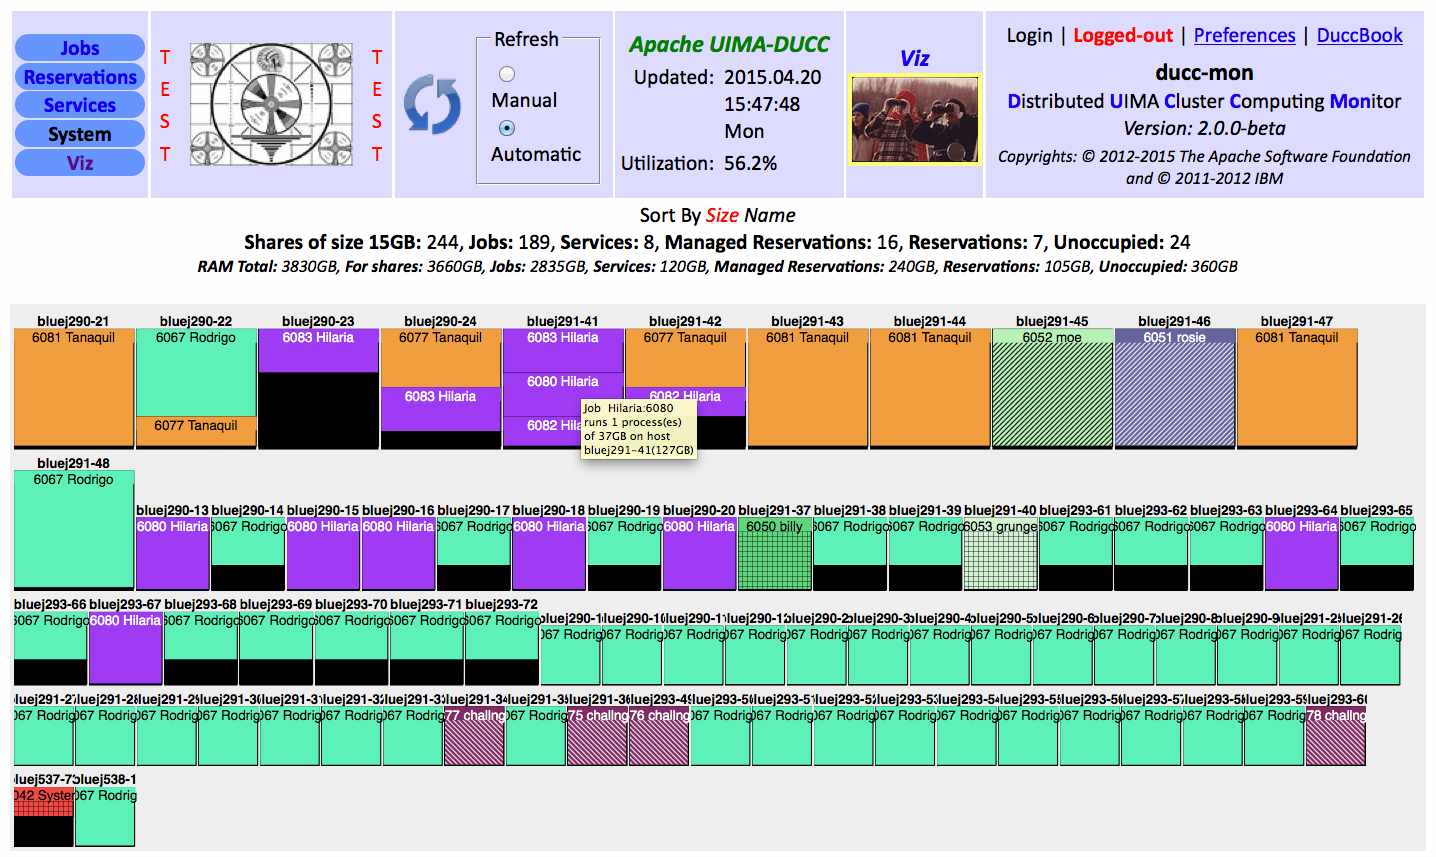
\includegraphics[width=160mm]{images/ducc-webserver/viz.jpg}
    \caption{Visualization}
    \end{figure}


